\chapter{$B_s\to D_s^*l\nu$ Axial Form Factor at Zero Recoil from Heavy-HISQ}
\label{chap:BsDsstar}

This chapter concerns the simpler of our two heavy-HISQ studies, the calculation of the $B_s\to D^*_sl\nu$ form factor at zero recoil, $h^s_{A_1}(1)$ as defined in Sec. \ref{sec:weakdecays}. We give this quantity the superscript $s$ to differentiate it from the quantity more commonly referred to as $h_{A_1}(1)$, the zero recoil axial form factor for $B\to D^*l\nu$ decays.

We breifly review the definition of this form factor (at zero recoil) for clarity. The differential decay rate for the $\bar{B}_s^0\to D_s^{*+} l^- \bar{\nu}_l$ decay is given in the SM by
\begin{align}
  {d \Gamma \over dw} &(\bar{B}_s^0\to D_s^{*+} l^- \bar{\nu}_l) = {G_F^2 M_{D_s^*}^3 | \eta_{\text{EW}} V_{cb} |^2 \over 4\pi^3}
\\  &\times(M_{B_s}^2-M_{D_s^*}^2) \sqrt{w^2-1} \chi(w) | \mathcal{F}^{B_s\to D_s^*}(w) |^2. \nonumber
\end{align}
where $w = v_{B_s} \cdot v_{D^*_s}$, $v_H = p_H/M_H$ is the 4-velocity of a $H$-meson, and $\chi(w)$ is a known function of $w$ (see appendix G of \cite{Harrison:2017fmw}). $\eta_{\text{EW}}$ accounts for electroweak corrections due to diagrams where photons or $Z$s are exchanged in addition to a $W^-$, as well as the Coulomb attraction of the final-state charged particles \cite{SIRLIN198283,Ginsberg1968,PhysRevD.41.1736}. The differential decay rate for the $B_s^0\to D_s^{*-} l^+ \bar{\nu}_l$ is identical.

The form factor $\mathcal{F}^{B_s\to D_s^*}(w)$ is a linear combination of hadronic form factors that parameterize the vector and axial-vector matrix elements between initial and final state hadrons. At zero recoil ($w=1$), the vector matrix element vanishes, the axial-vector element simplifies to
\begin{align}
  \langle D^*_s(\epsilon)| A^{\mu} | B_s \rangle &= 2 \sqrt{M_{B_s}M_{D^*_s}} h^s_{A_1}(1) \epsilon^{*\,\mu},
\end{align}
and $\mathcal{F}^{B_s\to D_s^*}(w)$ reduces to
\begin{align}
  \mathcal{F}^{B_s\to D_s^*}(1) = h^s_{A_1}(1).
\end{align}
Our goal is to compute $h^s_{A_1}(1)$.

All we need to do this is the matrix element $\langle D^*_s(\epsilon)| A^{\mu} | B_s \rangle$ with both the $B_s$ and $D_s^*$ at rest, with the $D_s^*$ polarization $\epsilon$ in the same direction as the axial current.

\section{Motivation}
\label{sec:BsDsstar_intro}

The $\bar{B}\to D^{*} l \bar{\nu}_l$ decay supplies one of the three methods used for precisely determining the CKM element $|V_{cb}|$ \cite{Schroder:1994aj,PhysRevLett.64.2117,PhysRevD.43.651,ALBRECHT1992195,Barish:1994mu,BUSKULIC1996449,Buskulic:1994dz,Abbiendi:2000hk,Abreu:2001ic,Adam:2002uw,Abdallah:2004rz,Aubert:2007rs,Aubert:2007qs,Aubert:2008yv,Dungel:2010uk,Abdesselam:2017kjf,Bailey:2014tva,Abdesselam:2018nnh}.
Measurements of branching fractions are extrapolated through $q^2$ to the zero recoil point to deduce $h_{A_1}(1) |V_{cb}|$, where $h_{A_1}(1)$ is the only form factor contributing at zero recoil. Then an SM determination of $h_{A_1}(1)$ (via Lattice QCD \cite{Bailey:2014tva,Harrison:2017fmw}) can be divided out to infer $|V_{cb}|$.

A similar process that could also be used to determine $|V_{cb}|$, and test the SM, is $\bar{B}_s \to D^*_s l\bar{\nu}_l$. There is at time of writing no published measurements of this decay, but it is feasable to measure such a decay at a detector like LHCb. This decay is also attractive from the Lattice QCD side.

The absense of valence light quarks means lattice QCD results have smaller statistical errors, are less computationally expensive, a simpler chiral extrapolation to the physical light mass, and negligable finite volume effects. This makes the $\bar{B}_s \to D^*_s l\bar{\nu}_l$ both a useful test bed for lattice techniques (that may be later used to study $\bar{B} \to D^* l \bar{\nu}_l$ decays), and a key decay to make predictions about for when experimental results become available.

Chiral symmetry implies that form factors for decays such as $B_s \to D^*_s$ and $B \to D^*$ are insensitive to the mass of the spectator quark, since  implying that form factors for these two decays are approximately equal \cite{Laiho:2005ue}. This was seen in the recent lattice calculation \cite{Harrison:2017fmw} that found $h_{A_1}^{B_s\to D_s^*}(1) / h_{A_1}^{B\to D^*}(1) = 1.013(14)_{\text{stat}}(17)_{\text{sys}}$. We can then expect to learn about $B\to D^*$ by studying $B_s\to D_s^*$. We perform test of this claim, in the context of our formalism, in this study.

Lattice calculations of the $B_{(s)} \to D_{(s)}^*$ form factors at zero recoil have so far been performed by two collaborations. The Fermilab Lattice collaboration produced $h_{A_1}^{B\to D^*}(1)$ in \cite{Bailey:2014tva}. HPQCD computed both $h_{A_1}^{B\to D^*}(1)$ and $h_{A_1}^{B_{s}\to D_{s}^*}(1)$ in \cite{Harrison:2017fmw}. The RBC/UKQCD \cite{Flynn:2016vej} and LANL-SWME \cite{Bailey:2017xjk} collaborations are also working towards these form factors.

%% Lattice calculations of the $B_{(s)} \to D_{(s)}^*$ form factors at zero recoil have been performed by a number of collaborations. RBC/UKQCD is working towards determining the form factors using their 2+1 gauge ensembles, Domain Wall light, strange and charm quarks, and Wilson-type bottom quarks \cite{Flynn:2016vej}. The FNAL/MILC collaboration produced the $B\to D^*$ form factor at zero recoil on the 2+1 MILC ensembles using ASQTAD light and strange quarks and Wilson-type charm and bottom quarks \cite{Bailey:2014tva}. HPQCD has produced $B_{(s)}\to D_{(s)}^*$ form factors at zero recoil, on the 2+1+1 MILC ensembles, HISQ light, strange and charm quarks, and NRQCD bottom quarks \cite{Harrison:2017fmw}.

The presence of heavy quarks is a large consideration in designing a lattice calculation. A $b$ quark introduces discretization effects of size $(am_b)^n$ where $n$ is a positive integer dependent on the choice of action. To avoid such potentially large discretization effects, most lattice studies (including all of those mentioned in the previous paragraph), use some EFT approach for simulating heavy quarks. The Fermilab Lattice, RBC/UKQCD, and LANL-SWME calculations all use some variation of the Fermilab action \cite{Wilson:1977xx,SHEIKHOLESLAMI1985572,ElKhadra:1996mp} to simulate $c$ and $b$ quarks. The HPQCD calculation uses the NRQCD action \cite{Lepage:1992tx} for $b$ quarks. 

To relate the results from these approaches to full continuum QCD, each of the above studies requires perturbative matching of lattice currents to continuum QCD. The matching has only been performed to 1-loop, leading to each having matching errors as a key uncertainty. The use of NRQCD in the HPQCD calculation brings in matching errors of $\order{\alpha_s^2,\alpha_s \Lqcd / m_b, (\Lqcd / m_b )^2}$. It is difficult to estimate the size of matching errors in lattice NRQCD, so to be conservative a large matching error was assigned to the result. This error contributes $\sim 80\%$ of the full error budget. The use of the Fermilab action in the Fermilab Lattice calculation leads to $\order{\alpha_s^2}$ errors. They avoid this issue to a large extent by analysing only ratios of correlation functions, however, the matching still contributes $\sim 30\%$ to the final error. %The final results for the RBC/UKQCD calculation are not yet published, however, they report requiring matching factors that are only known to tree level, which could cause errors as large as $\order{\alpha_s}$ in the final result.

In this chapter, we report details and results of the first calculation of the $B_s\to D^*_s$ form factor at zero recoil using an approach free of perturbative matching. 

Since the $B_s\to D_s$ form factor is approximately equal to the $B\to D$ form factor, and our results are non-perturbatively renormalised, this calculation can be seen as a check of the normalisation of the Fermilab Lattice and HPQCD determinations of $h_{A_1}(1)$ that contributed to $|V_{cb}|_{\text{excl}}$. While producing a quantity less relevant to current phenomenology than the $B\to D^*$ form factor, this calculation can be seen as a proof-of-principle for the heavy-HISQ approach. 

Using the heavy-HISQ approach has the added benefit of eludicating the dependence of form factors on heavy quark masses, meaning we can test expectations from Heavy Quark Effective Theory (HQET). In this article we give a determination of the HQET low energy constants $l_{V,A,P}^s$ associated with the $B_s \to D_s^*$ form factor at zero recoil.

\section{Calculation Details}
\label{sec:BsDsstar_deets}

\subsection{Lattice Setup}

We use the MILC gluon field configurations detailed in Sec. \ref{sec:MILCensembles} \cite{Bazavov:2010ru,Bazavov:2012xda}. We use sets 2-5 in table \ref{tab:ensembles}, i.e., the fine, fine-physical, superfine and ultrafine ensembles. Table \ref{tab:BsDsensembles} gives the valence quark masses we use in the generation of quark propagators. In three of the four ensembles (fine,superfine and ultrafine), the bare light mass is set to $m_{l0}/m_{s0} = 0.2$. The fact that the $m_{l0}$ value is unphysically high is expected to have a small effect on $h^s_{A_1}(1)$, due to the lack of valence light quarks, and previous experience of the dependence of $h_{A_1}^s(1)$ on $m_{l0}$ \cite{Harrison:2017fmw}. The small effect due to the unphysical $m_{l0}$ is quantified by including a fourth ensemble (fine-physical) with physical $m_{l0}$, and corrected for.

We use a number of different masses for the valence heavy quark. This is in order to resolve the dependence of $h_{A_1}^s(1)$ on the heavy mass, so that an extrapolation to $m_h=m_b$ can be performed. By varying the heavy mass varying both within ensembles and between ensembles, we can resolve both the discretization effects that grow with large ($am^{\text{val}}_{h0} \lesssim 1$) masses and the physical dependence of the continuum form factor on $m_h$.

\begin{table}
  \begin{center}
    \begin{tabular}{c c c c c c}
      \hline
      set & handle & $am_{s0}^{\text{val}}$ & $am_{c0}^{\text{val}}$ & $am^{\text{val}}_{h0}$ & T \\ [0.5ex]
      \hline
      2 & \bf{fine} & 0.0376 & 0.45 
      & 0.5, 0.65, 0.8 & 14,17,20 \\ [1ex]
      3 & \bf{fine-physical} & 0.036 & 0.433 
      & 0.5, 0.8 & 14,17,20 \\ [1ex]
      4 & \bf{superfine} & 0.0234 & 
      0.274 & 0.427, 0.525, 0.65, 0.8  & 22,25,28  \\ [1ex]
      5 & \bf{ultrafine} & 0.0165 
      & 0.194 & 0.5, 0.65, 0.8 & 31,36,41\\ [1ex]
      \hline
    \end{tabular}
  \end{center}
  \caption{Parameters relevent to our calculation. Columns 3 and 4 give the $s$ and $c$ valence quark masses, these values were tuned in \cite{Chakraborty:2014aca} to reproduce the correct $\eta_s$ and $\eta_c$ masses. We use a number of heavy quark masses to assist the extrapolation to physical the $b$ mass, given in column 5. Column 6 gives the temporal separations between source and sink, $T$, of the 3-point correlation functions computed on each ensemble.}
  \label{tab:BsDsensembles}
\end{table}

As detailed in Sec. \ref{sec:staggeredcorrelators}, staggered correlation functions are built by a combination of staggered propagators $g(x,y)$ and staggered phases. In this calculation we only need local (non point-split) operators, this is an advantage since point-split operators lead to correlation functions more noisy than local operators. 

We compute a number of correlation functions on each ensemble. To generate these correlators we use random wall sources, and use extended sources for the 3-point correlators, as described in Sec. \ref{sec:staggeredcorrelators}. First we compute 2-point correlation functions between zero-momentum eigenstates, objects of the form
\begin{align}
  C_{M}(t) =& \langle \Phi_M (t) \Phi_M^{\dagger}(0) \rangle, \\ 
  &\Phi_M(t) = \sum_{{\bf{x}}} \bar{q}({\bf{x}},t) \Gamma q'({\bf{x}},t), \nonumber
\end{align}
where $\langle \rangle$ represents a functional integral, $q,q'$ are valence quark fields of the flavours the $M$ meson is charged under, and $\Gamma$ is the spin-taste structure of $M$. We compute these for all $t$ values, i.e. $0\leq t \leq N_t$. 

We compute correlation functions for a heavy-strange pseudoscalar, $H_s$, with spin-taste structure $(\gamma_5\otimes \gamma_5)$. In terms of staggered propagators this takes the form
\begin{align}
  C_{H_s}(t) = \sum_{\bf{x},\bf{y}} \text{Tr}\left[ g_h(x,y) g_s^{\dagger}(x,y) \right],
  \label{eq:pseudoscalar_corrs}
\end{align}
where $g_q(x,y)$ is a staggered propagator for flavour $q$, and the trace is over color. Here $x_0=0$ and $y_0=t$, and the sum is over spacial sites {$\bf{x}$, $\bf{y}$}. We also compute correlators for a charm-strange vector meson $D_s^*$, with structure $(\gamma_{\mu}\otimes \gamma_{\mu})$, using
\begin{align}
  C_{D_s^*}(t) = \sum_{\bf{x},\bf{y}} (-1)^{x_{\mu}+y_{\mu}}\text{Tr}\left[ g_c(x,y) g_s^{\dagger}(x,y) \right].
\end{align}

In order to non-perturbatively renormalise the axial vector current, we compute correlation functions for goldstone and non-goldstone pseudoscalar and heavy-charm mesons denoted $H_c$ and $\hat{H}_c$ respectively, where $H_c$ has spin-taste structure $\Gamma_P$, and $\hat{H}_c$ has structure $\Gamma^0_A$. $H_c$ correlators are computed using \eqref{eq:pseudoscalar_corrs} (with $g_s$ replaced with $g_c$), while $\hat{H}_c$ correlators are given by
\begin{align}
  C_{\hat{H}_c}(t) = \sum_{\bf{x},\bf{y}}(-1)^{\bar{x}_0+\bar{y}_0} \text{Tr}\left[ g_h(x,y) g^{\dagger}_c(x,y) \right],
\end{align}
where we use the notation $\bar{z}_{\mu} = \sum_{\nu\neq\mu} z_{\nu}$.

The heavy-mass extrapolation requires masses of $\eta_h$ mesons, heavy-heavy pseudoscalars artificially forbidden to annihilate. To quantify mistuning of the charm and strange quark masses, we also require masses for $\eta_c$ and $\eta_s$ mesons, identical to $\eta_h$ with $h$ replaced $c$ and $s$ quarks respectively. We compute correlators for each of these, using a spin-taste $(\gamma_5\otimes \gamma_5)$, taking the form of \eqref{eq:pseudoscalar_corrs}.

We then generate the 3-point correlation functions
\begin{align}
  C_3(t,T) =& \sum_{{\bf{y}}} \langle \Phi_{D_s^*(\epsilon)}(T)\, A^{\mu}({\bf{y}},t) \,\Phi_{H_s}(0) \rangle, \\
  &A^{\mu}({\bf{y}},t) = \bar{c}({\bf{y}},t) \gamma^5\gamma^{\mu} h({\bf{y}},t). \nonumber
\end{align}
In terms of the staggered formalism, the $H_s$ source is given structure $(\gamma_5\otimes \gamma_5)$, the $D_s^*$ sink is given $(\gamma_{\mu}\otimes \gamma_{\mu})$, and the current insertion $(\gamma_5\gamma_{\mu}\otimes \gamma_5\gamma_{\mu})$. In terms of staggered propagators this is given by
\begin{align}
  C_3(t,T) =& \sum_{{\bf{x},\bf{y},\bf{z}}} (-1)^{\bar{y}_{\mu}+\bar{z}_{\mu}}  \nonumber \\ &\times\text{Tr}\left[ g_h(x,y)g_c(y,z) g^{\dagger}_s(x,z) \right],
\end{align}
where we fix $x_0 = 0$, $y_0=t$ and $z_0=T$. We compute these for all $t$ values within $0\leq t\leq T$, and 3 $T$ values that vary between ensembles, given in table \ref{tab:BsDsensembles}.

In the $C_{D_s^*}$ and $C_3$ cases, dependant on a polarization $\mu$, we compute the cases with $\mu = x,y,z$, and take the average over these.

\subsection{Correlator Fits}

We extract current matrix elements from the generated correlation functions, via simultaneous Bayesian fits as described in Sec. \ref{sec:correlator_fits}. We use fit forms given by \eqref{eq:2ptcorrelator_real} for 2-point and \eqref{eq:3ptcorrelator_real} for 3-point correlators. We set $N_{\text{exp}}=5$ is each fit. We perform a single simultanious fit containing each correlator computed ($H_s,D_s^*,\eta_h,\eta_s,H_c,\hat{H}_c$, and 3-point) for each ensemble. We also marginalize out the highest energy excited states in the fit function using the prior distributions, in the interest of speed of the fits.

We set gaussian priors for the parameters $J_{jk}$, and log-normal priors for all other parameters. Using log-normal distributions forbids energies $E_n^M$ and amplitudes $a_n^M$ from moving arbitrarily close to zero, improving stability of the fit.

Ground state energies $E_0^M$ are given priors of $(am_{q0} + am_{q'0} + a\Lambda_{\text{QCD}} )\pm 2a\Lambda_{\text{QCD}}$, where $m_{q0,q'0}$ are the masses of the flavours the meson $M$ is charged under, and $\Lambda_{\text{QCD}}$ is the confinement scale, which we set to 0.5GeV. For $q=h$ or $c$, this corresponds to the leading order HQET expression for a heavy meson mass. In the $\eta_s$ case, the prior becomes approximately $2am_{s0} + a\Lambda_{\text{QCD}} \simeq a\Lambda_{\text{QCD}}$, which one would expect. Ground-state energies of oscillaing states, $E_0^{M,o}$, are given priors of $(am_{q0} + am_{q'0} + 2 a\Lambda_{\text{QCD}})\pm 2\Lambda_{\text{QCD}}$. Excited state energies, $E_i^M$, $i>0$ are given prior values $2a\Lambda_{\text{QCD}}\pm a\Lambda_{\text{QCD}}$. Priors for ground state amplitudes $a_0^M$, are set according to an empirical-Bayes approach, plots of the effective applitude of the correlation functions are inspected to deduce reasonable priors. The resulting priors always have a variance at least 10 times that of the final result. The excited state amplitudes $a_i^M$,$i>0$ are given priors of $0.15\pm 0.5$ for non-oscillating states, and $0.05\pm 0.1$ for oscillating states. The ground-state non-oscillating to non-oscillating 3-point parameter, $J_{00}^{nn}$ is given a prior of $1\pm 0.6$, and the rest of the 3-point parameters $J_{jk}^{nn}$ are given $0\pm 1$.

The current matrix element we require to find $h_{A_1}^s(1)$ is given by
\begin{align}
  \langle D_s^*(\hat{k}) | A^k | H_s \rangle |_{\text{lat}} = 2 \sqrt{M_{H_s}M_{D_s^*}} J^{nn}_{00}.
  \label{eq:currentfit}
\end{align}

We performed a number of tests on the fits, to demonstrate the robustness of the fits to various hyperparameter choices. Results are given in fig. \ref{sec:correlator_fits}. We will refer to these tests throughout the remainder of this section. In test $\#1$ we loosened priors to test stability. We tested the effects of changing $N_{\text{exp}}$, to $N_{\text{exp}}=6$ in test $\#2$ and $N_{\text{exp}}=4$ in test $\#3$.

\begin{figure}[htb!]
  \begin{center}
  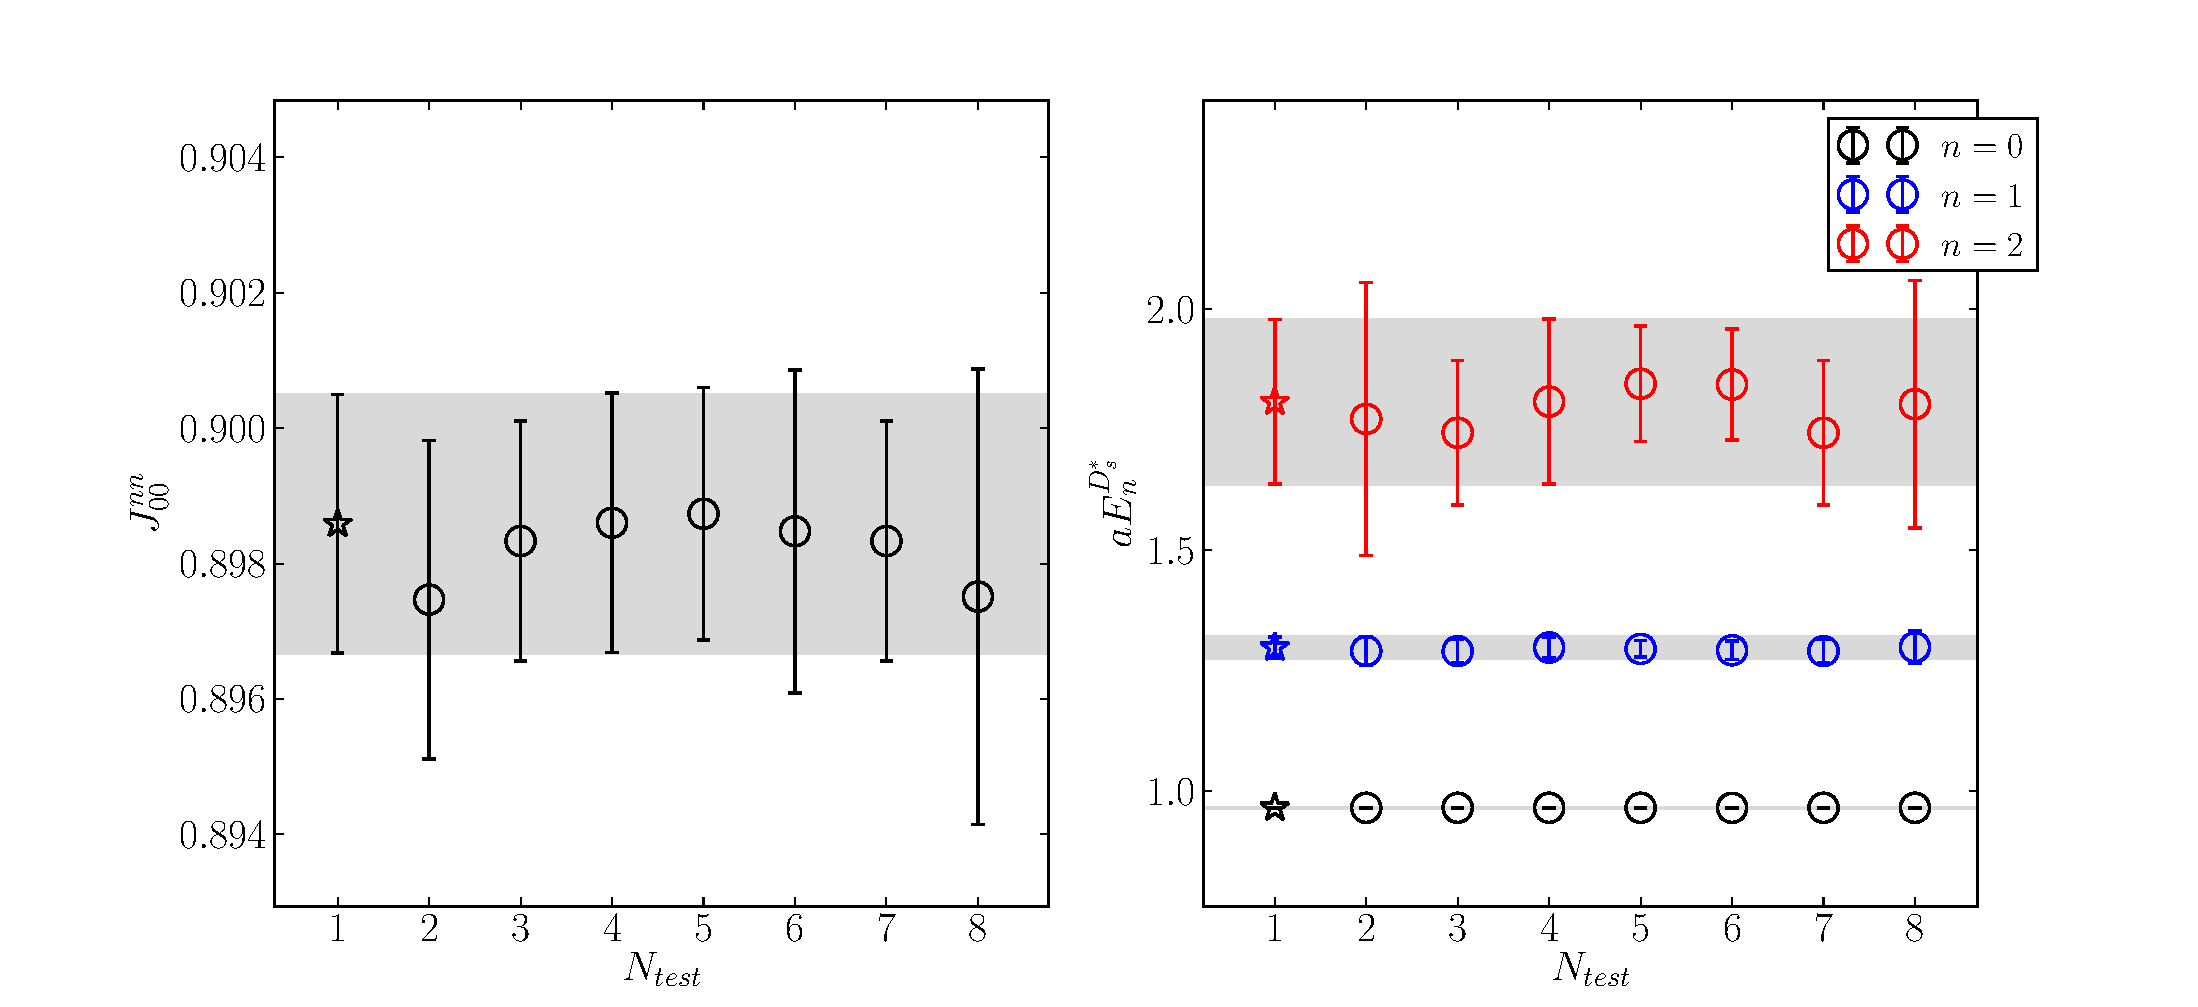
\includegraphics[width=1.1\textwidth]{images/BsDsstar/fittests_fine.pdf}
  \caption{Tests on the correlator fits on the fine ensemble. At $N_{\text{test}}=1$ we give the final accepted result. $N_{\text{test}}=2$ gives the results when all priors are loosened by 50\%. $N_{\text{test}}=3$ and $4$ gives the results of setting $N_{\text{exp}}=4$ and $6$ respectively. $N_{\text{test}}=5,6$ gives the results of setting $t_{\text{cut}}=2,4$ respectively for all correlators. $N_{\text{test}}=7$ gives the result without marginalising out the $n=5$ excited state. $N_{\text{test}}=8$ gives the result of moving the SVD cut from $10^{-3}$ to $10^{-2}$. \label{fig:corr_fit_tests}}
  \end{center}
  \vspace{-10pt}
\end{figure}

To ensure that truncating the sum at $N_{\text{exp}}$ is a good approximation to the infinite sum containing all excited states, we only include data with  $t \geq t_{\text{cut}}$ and $t \leq N_t-t_{\text{cut}}$ in the 2-point case and $t \leq T-t_{\text{cut}}$ in the 3-point case. We can in principle use a different $t_{\text{cut}}$ for every correlation function included in our fit, so must choose a set $\{ t_{\text{cut}}^{c}\}$ (where $c$ labels the correlator).

To ensure the optimal choice for the $\{ t_{\text{cut}}^{c}\}$ set, we employ the \texttt{scikit-optimize} python package \cite{skopt}. The process consists of defining a function $f$ with an input of $\{ t_{\text{cut}}^{c}\}$ and an output of some loss function $f$. Then, the minimum of $f$ with respect to $\{ t_{\text{cut}}^{c}\}$ is found via a Gaussian process. We use the loss function
\begin{align}
  f(\{ t_{\text{cut}}^{c}\}) = - \log \text{GBF} + \theta\left({\chi^2\over N_{\text{dof}}}-1\right) \,\rho\, {\chi^2\over N_{\text{dof}}}.
\end{align}
GBF is the Gaussian Bayes factor corresponding to the comparison between the resulting model of the fit (the fit function with parameters set by the fit), and a random model (the fit function with randomly sampled parameters). The second term gives a strong punishment to fits with $\chi^2/N_{\text{dof}} > 1$. We set $\rho=10^5$, in order to make the second term of comparable size of the first, which for typical fits we attemtped had a magnitude of order $10^4$. A couple of more naive choices for $\{ t_{\text{cut}}^{c}\}$ are given in tests $\#3 \,\&\, \#4$.

An appropriate value for the SVD-cut is found by comparing estimates of covariance matrix eigenvalues between different bootstrap samples of the data. Typically the smallest eigenvalues are sensitive to taking new bootstrap copies, suggesting they are poorly estimated. A cut is placed such that any poorly estimated eigenvalues are replaced with more conservative (larger) values. The resulting SVD cut varies between ensembles since it depends on the quality of the dataset, but are always of order $10^{-3}$.

Fig. \ref{fig:svddiagnosis_BsDsstar} illustrates this process on the fine ensemble. In fits to the fine ensemble correlators, we set the SVD cut to $10^{-3}$, we then tested to see if this had any effect by also running the fit with SVD cut $10^{-2}$ in test \#7.

\begin{figure}[htb!]
  \begin{center}
  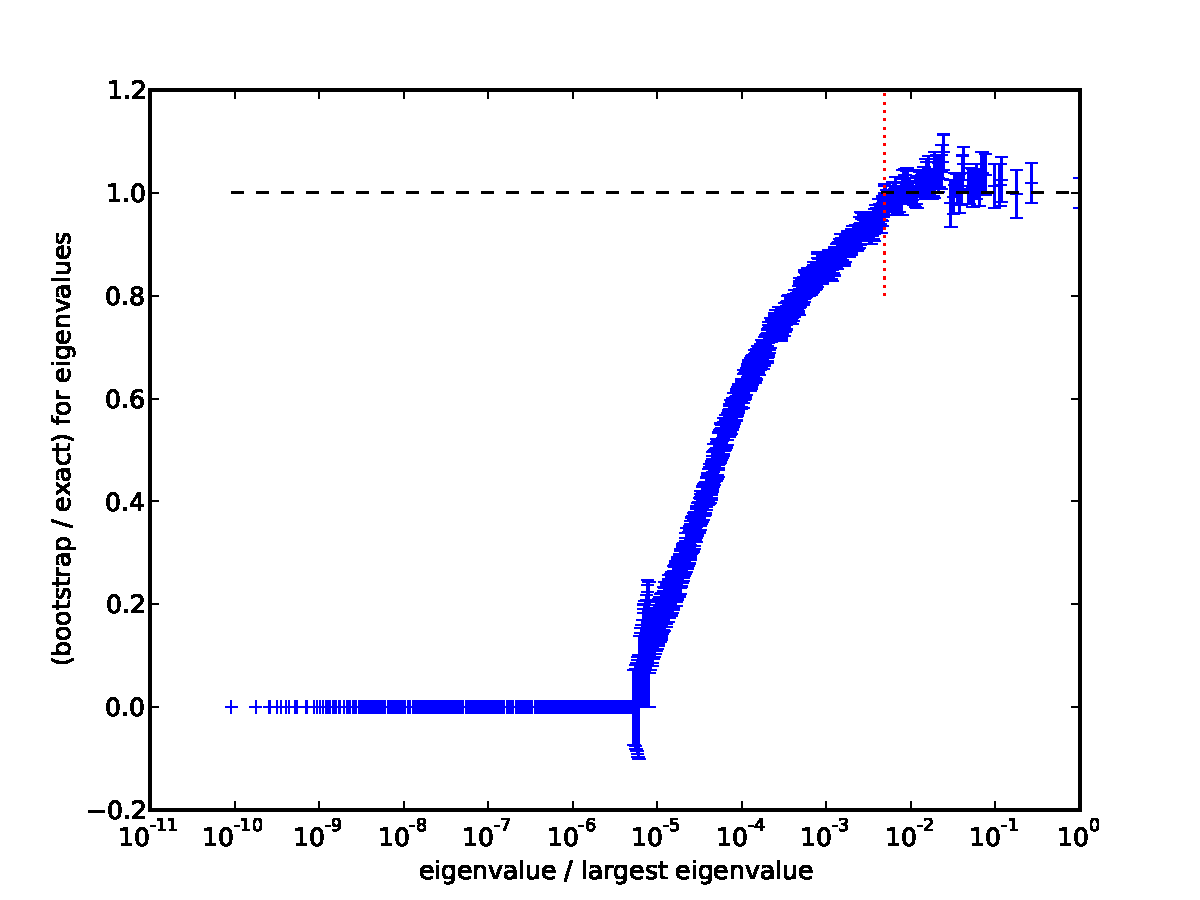
\includegraphics[width=0.8\textwidth]{images/BsDsstar/svddiagnosis_fine.pdf}
  \caption{An illustration of the process of deducing an appropriate SVD cut on the fine ensemble. Each point shows the ratio of a covariance matrix eigenvalue, to the same eigenvalue from a bootstrap copy, against the relative size of the eigenvalue. The eigenvalues below the red dotted line are at risk of being underestimated. \label{fig:svddiagnosis_BsDsstar}}
  \end{center}
  \vspace{-10pt}
\end{figure}

We can perform further sanity checks on the fits by plotting certain functions of the 2-point correlators. To obtain useful forms, first, one can approximately flush out the oscillating states from correlators by performing a so-called {\it{superaverage}}, $C(t) \to [ C(t) + C(t+a) ]/2$. We perform a symmetric and doubled version of this operator on correlators to obtain
\begin{align}
  C(t) \to \tilde{C}(t) = {1\over 4}( C(t-a) - 2C(t) + C(t+a) ).
  \label{eq:superav2}
\end{align}
We can check the ground-state energy of the correlator by looking at the large-$t$ behaviour of
\begin{align}
  E_{\text{eff}}(t) = \log\left({ \tilde{C}(t)\over \tilde{C}(t-a) }\right).
  \label{eq:effectivemass}
\end{align}
It is straightforward to show from inspecting eq. \eqref{eq:multiexponential} that in the large $t$ (but $t < T_{\text{lat}}/2$) limit, this should tend towards the ground-state energy for the correlator. One can also construct a similar function for the amplitude:
\begin{align}
  a_{\text{eff}}(t) = \sqrt{\cosh E_{\text{eff}}(t)-1\over 2} \sqrt{ \tilde{C}(t) e^{E_{\text{eff}}t} }.
  \label{eq:effectiveamp}
\end{align}
The second term would produce the correct amplitude (in the large-$t$ limit) in the absence of superaveraging, and the first corrects for the effect of the superaveraging \eqref{eq:superav2}. These functions, for various relevant correlators on the fine ensemble, are plotted in comparison with the full fit results in fig. \ref{fig:2pt-summary_BsDsstar}.

\begin{figure}[htb!]
  \begin{center}
  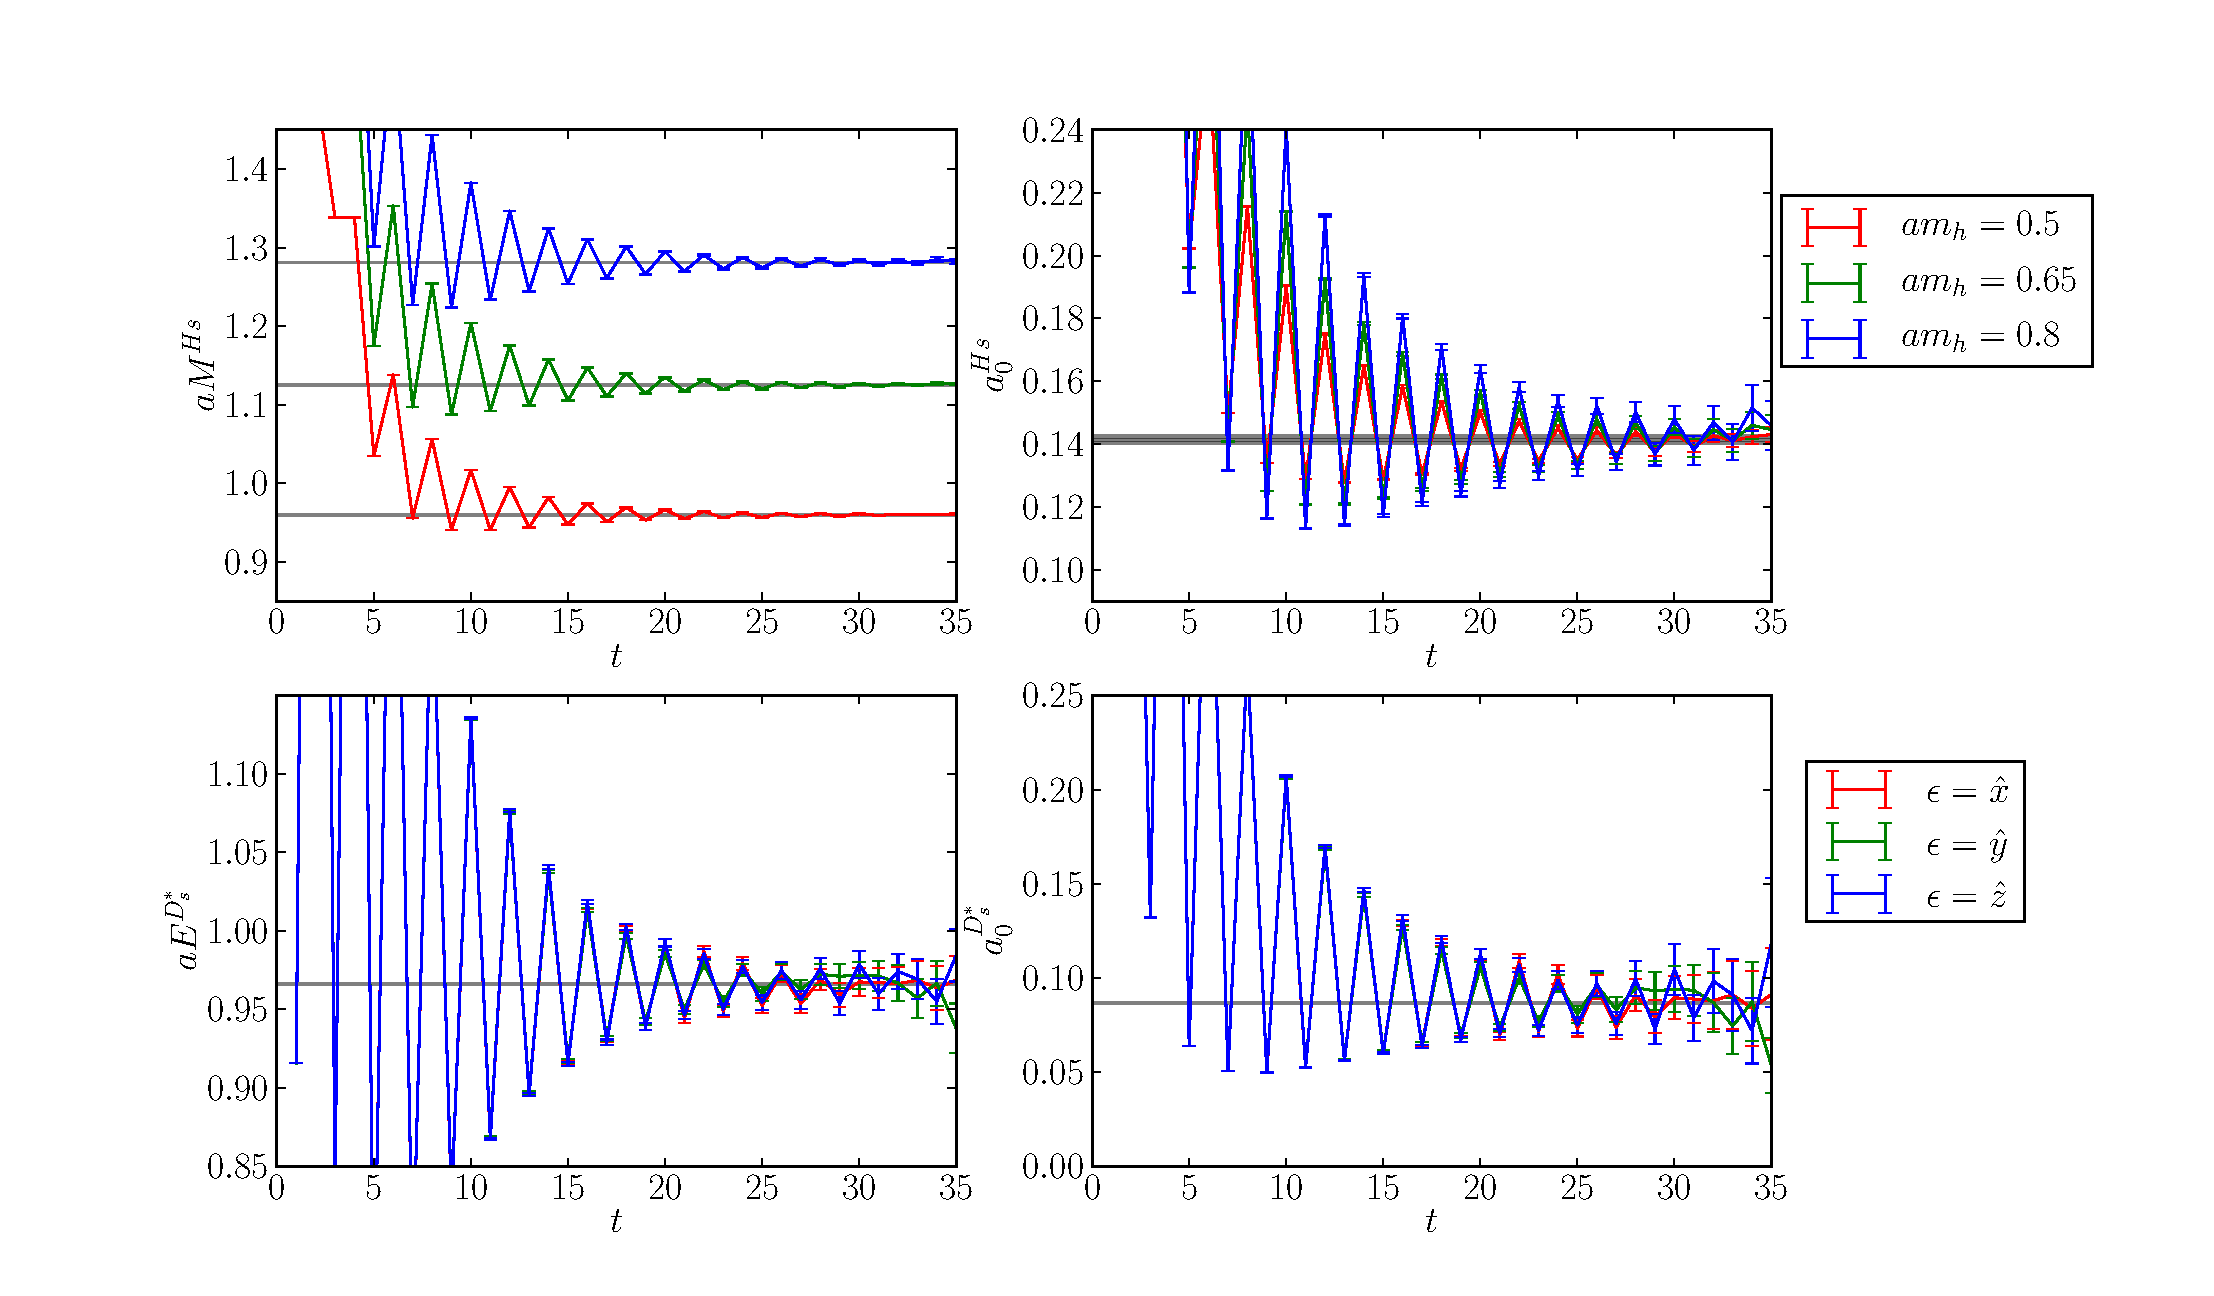
\includegraphics[width=1.1\textwidth]{images/BsDsstar/2ptsummary_fine.pdf}
  \caption{Effective energies and amplitudes for $H_s$ and $D_s^*$ correlators on the fine ensemble. The energies are obtained from eq. \eqref{eq:effectivemass}, and amplitudes from eq. \eqref{eq:effectiveamp}. The grey bands give the results of the full multiexponental fit. \label{fig:2pt-summary_BsDsstar}}
  \end{center}
\end{figure}

A similar approach can be applied to the 3-point correlators. The ratio $\tilde{C}_3(t,T)/\tilde{C}^{H_s}(t) \tilde{C}^{D_s^*}(T-t)$ approaches $J_{00}^{nn}$ for $t>>0$ and $t<<T$. This is illustrated in fig. \ref{eq:3pt-summary_BsDsstar}. From inspecting these figures for 2- and 3-point sanity tests, one can reassure themselves that the fits to the correlators are well behaved.

\begin{figure}[htb!]
  \begin{center}
    \vspace{-10pt}
  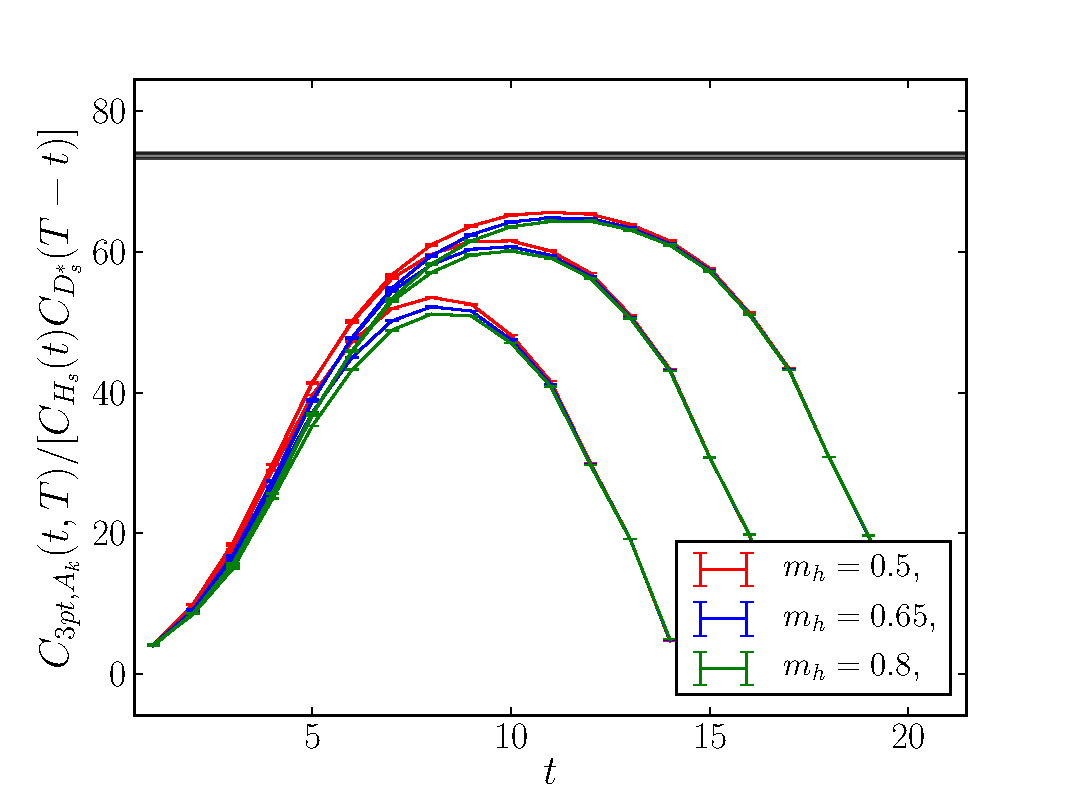
\includegraphics[width=0.8\textwidth]{images/BsDsstar/3ptsummary_fine.pdf}
  \caption{Sanity check for fits to the 3-point correlation functions. This ratio should approach $J_{00}^{nn}$ for $t>>0$ and $t<<T$. The grey band shows the result for $J_{00}^{nn}$ from the full multiexponential fit. \label{eq:3pt-summary_BsDsstar}}
  \end{center}
  \vspace{-10pt}
\end{figure}

\subsection{Normalization of Axial Current}

Conserved and partially conserved currents require no renormalization. However, the staggered conserved axial-vector current is not simply $(\gamma_5\gamma_{\mu}\otimes \gamma_5\gamma_{\mu})$, it is a complicated linear combination of many local and point-split lattice currents. In this study we use only local axial vector currents, this simplifies the lattice calculation but creates the need for our resulting current matrix element to be multiplied by a matching factor $Z_A$ to produce the appropriate continuum current. We find $Z_A$ via a fully non-perturbative method \cite{McNeile:2011ng,Donald:2013pea}.

We leverage the fact that the staggered local pseudoscalar current $(\gamma^5\otimes \gamma^5)$, multiplied by the sum of masses of quark flavours the current is charged under, is absolutely normalized. We extract from the 2-point $H_c$ and $\hat{H}_c$ correlators the decay amplitudes $\langle \Omega | \bar{c} (\gamma_5\otimes \gamma_5) h | H_c \rangle \equiv \langle \Omega | P | H_c \rangle$, $\langle \Omega | \bar{c} (\gamma_0\gamma_5 \otimes \gamma_0\gamma_5) h | \hat{H}_c \rangle = \langle \Omega | A_0 | \hat{H}_c \rangle$. Then, the normalization for $A_0$ (common to that of spacial axial currents $A_k$) $Z_A$, is fixed by demanding that the partially conserved axial current relation holds-
\begin{align}
  (m^{\text{val}}_{h0} + m^{\text{val}}_{c0}) \langle \Omega | P | H_c \rangle|_{\text{lat}} = M_{\hat{H}_c} Z_A \langle \Omega | A^0 | \hat{H}_c \rangle|_{\text{lat}}.
  \label{eq:ward}
\end{align}
The $Z_A$ values found on each ensemble and $am^{\text{val}}_{h0}$ are given in table \ref{tab:norms}.

There is an ambiguity in what mass to use on the right hand side of \eqref{eq:ward}, we here use the non-goldstone mass $M_{\hat{H}_c}$, but one could just as well replace this with $M_{H_c}$. Using $M_{H_c}$ here changes $Z_A$ only by discretization effects, the difference never exceeding 0.0015 throughout the ensembles and heavy masses. The choice between these two definitions of $Z_A$ does not effect the continuum result.

We also remove tree-level mass-dependent discretization effects, at leading order in $|{\bf{p}}_h|/m_h$, using a normalization constant derived in \cite{Bazavov:2017lyh}:
\begin{align}
  \label{eq:Zdisc}
  Z_{\text{disc}} &=\,\sqrt{ \tilde{C}_h \tilde{C}_c }, \\
  \nonumber
  &\tilde{C}_q = \cosh am_{q1} \left( 1 - {1-\epsilon_{\text{Naik}}\over 2} \sinh^2 am_{q1} \right), \\ \nonumber
  &am_{q1} = am_{q0} \Big( 1 - {3\over 88}am_{q0}^4 + {23\over 2240}am_{q0}^6 \\ \nonumber
  &+ {1783\over 537600} am_{q0}^8 - {76943\over23654400}am_{q0}^{10} + \order{am_{q0}^{12}} \Big), \nonumber
\end{align}
where $\epsilon_{\text{Naik}}$ is the Naik parameter in the HISQ action and $am_{q1}$ is the tree-level pole mass in HISQ. The expansion for $am_{q1}$ in terms of $am_{q0}$ was derived in \cite{Follana:2006rc}. The effect of $Z_{\text{disc}}$ is very small, never exceeding $0.2\%$. $Z_{\text{disc}}$ values on each ensemble for each $am^{\text{val}}_{h0}$ are given in table \ref{tab:norms}.

Combining these normalizations with the lattice current from the 3-point fits, we find a value for the form factor at a given heavy mass and lattice spacing:
\begin{align}
  h_{A_1}^s(1) = {1\over 3} \sum_{k=0}^3 { Z_A Z_{\text{disc}}\langle D_s^*(\hat{k}) | A^k | H_s \rangle |_{\text{lat}}\over 2\sqrt{M_{H_s} M_{D_s^*}} }.
  \label{eq:normalizations}
\end{align}

\begin{table}
  \begin{center}
    \begin{tabular}{ c c c c }
      \hline
      Set & $am^{\text{val}}_{h0}$ & $Z_A$& $Z_{\text{disc}}$\\ [0.5ex]
      \hline
      2 & 0.5 & 1.03178(57) & 0.99819\\ [0.5ex]
      & 0.65 & 1.03740(58) & 0.99635\\ [0.5ex]
      & 0.8 & 1.04369(56) & 0.99305\\ [0.5ex]
      \hline
      3 & 0.5 & 1.03203(39) & 0.99829\\ [0.5ex]
      & 0.8 & 1.04389(38) & 0.99315\\ [0.5ex]
      \hline
      4 & 0.427 & 1.0138(11) & 0.99931\\ [0.5ex]
      & 0.525 & 1.0170(12) & 0.99859\\ [0.5ex]
      & 0.65 & 1.0213(12) & 0.99697\\ [0.5ex]
      & 0.8 & 1.0272(12) & 0.99367\\ [0.5ex]
      \hline
      5 & 0.5 & 1.00898(45) & 0.99889\\ [0.5ex]
      & 0.65 & 1.01365(50) & 0.99704\\ [0.5ex]
      & 0.8 & 1.01970(55) & 0.99375\\ [0.5ex]
      \hline
    \end{tabular}
    \caption{Normalization constants applied to the lattice axial vector current in \eqref{eq:normalizations}. $Z_A$ is found from \eqref{eq:ward} and $Z_{\text{disc}}$ from \eqref{eq:Zdisc}. \label{tab:norms}}
  \end{center}
\end{table}

\subsection{Extrapolation to Physical Point}
\label{sec:BsDsstar_extrapolation}

We now address the extrapolation of the $h_{A_1}^s(1)$ values to continuum and physical $b$ and $l$ masses. In the process of the extrapolation, we also aim to determine the HQET low energy constants $l^s_{V,A,P}$. This process requires a number of considerations.

\subsubsection{Heavy Mass Dependence}
\label{sec:BsDsstar_heavymass}

Our extrapolation in the $m_h$ direction can be guided by HQET. The HQET expression for $h^s_{A_1}(1)$ (where here we consider both $h$ and $c$ to be heavy quarks in the HQET context) is given by \cite{Falk:1992wt,Mannel:1994kv}:
\begin{align}
  \label{eq:hqet}
  h_{A_1} &= \eta_A \left( 1 - {l_V\over (2m_c)^2} + {2l_A \over 2 m_c m_h} - { l_P \over (2m_h)^2 } \right)  \\ \nonumber &+ \mathcal{O}\left( \, {1\over m_c^n m_h^m}, \, n+m\geq 3 \, \right).
\end{align}
$\eta_A$ accounts for matching between HQET and QCD, and has been computed at 2-loop: $\eta_A = 0.960(7)$ \cite{PhysRevLett.76.4124}. It is dependent on $m_h$, so one may worry that, if we are going to use this expression for the extrapolation in $m_h$, we must account for the $m_h$ dependence in $\eta_A$. However this dependence is weak in the region of $m_h$ we are interested in ($m_c \leq m_h \leq m_b$). This can be seen by examining how the 1-loop expression for $\eta_A$ varies with $m_h$ \cite{PASCHALIS1983473}:
\begin{align}
  \eta_A(m_h) = 1 - {3 \alpha_s(m_b) \over 4\pi} \left( {m_h+m_c\over m_h-m_c} \log\left({m_c\over m_h}\right) - 2 \right).
\end{align}
Fig. \ref{fig:etaAV} shows the variation of $\eta_A$ throughout this range; the value changes by around 1\%, This is negligable in relation to the errors we find in the parameters govorning the slope, $l_{V,A,P}$. so we can safely ignore the $m_h$ dependence in $\eta_A$. The fit was attempted with an extra factor multiplying $\eta_A$ of $(1+\rho \log(M_{\eta_c}/M_{\eta_h}))$, where $\rho$ was a free fit parameter, and this caused the Bayes factor to drop by a factor of 25. This implies that our lattice data cannot resolve any logarithmic behaviour in $m_h$, and we can safely ignore $\eta_A$'s $m_h$ dependence.

\begin{figure}[htb!]
  \begin{center}
  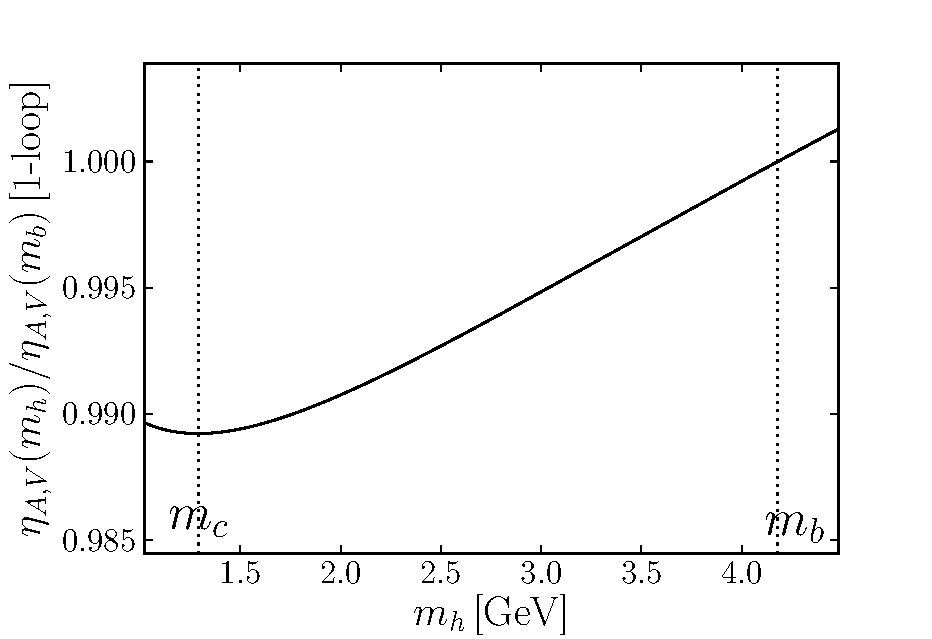
\includegraphics[width=0.6\textwidth]{images/BsDsstar/etaAV.pdf}
  \caption{The variation of the 1-loop expression for $\eta_{A}$ \& $\eta_V$ throughout the $m_c \leq m_h \leq m_b$ range. \label{fig:etaAV}}
  \end{center}
  \vspace{-10pt}
\end{figure}

\subsubsection{Quark Mass Ambiguities}
\label{sec:massambiguities}

If we are to determine $l_{V,A,P}^s$, attention must be paid to what to input for the masses $m_{h,c}$ in \eqref{eq:hqet}. Finding continuum quark masses corresponding to lattice bare masses would be a considerable task. Even if we took this on, what renormalisation scheme do the masses belong to? In HQET, the masses that define the power counting should be pole masses. Due to renormalons, the definition of pole masses is also ambiguous.

Thankfully, for our purposes, we do not need to worry about any of this. The quark masses in this equation can be replaced with expressions depending only on the meson masses $M_{H_s}$, $M_{D_s^*}$, which we can obtain for each ensemble and heavy mass from the $H_s$ and $D_s^*$ correlator fits.

To see this, first consider the HQET expansion of a heavy-light meson \cite{Bazavov:2018omf}:
\begin{align}
  \label{eq:hqet_mass}
  M_{H_q} = m_{h,S} + \bar{\Lambda}_S + { \mu^2_S \over m_{h,S}} + \mathcal{O}\left({1\over m_h^2}\right).
\end{align}
For notational brefity we are using the shorthand $\mu_S^2 = \mu^2_{\pi,S} - d_{H^{(*)}} \mu^2_{G,S}$, where $d_{H^{(*)}} = 1$ for pseudoscalar mesons and $-1/3$ for vectors. $\bar{\Lambda}_S,\mu_{\pi,S},\mu_{G,S}$ are HQET parameters and $q$ labels the light quark. As already mentioned, $m_h$ is defined in some renormalization scheme $S$, and since the meson mass $M_{H_q}$ is scheme-independent, the HQET parameters must also take on scheme dependence to cancel the dependence in $m_h$.

Changing the subject of eq. \eqref{eq:hqet_mass} to $m_h$ and taking the inverse, we find
\begin{align}
  \nonumber
  {1\over m_{h,S}} &= {1\over M_{H_q} - \bar{\Lambda}_S - { \mu^2_S \over m_{h,S}} } + \mathcal{O}\left({1\over m_h^2}\right), \\
  \nonumber
  &= {1\over M_{H_q} - \bar{\Lambda}_S} \left( 1 + { \mu^2_S \over  ( M_{H_q} - \bar{\Lambda}_S ) m_{h,S}} \right) + \mathcal{O}\left({1\over m_h^2}\right),
\end{align}
then solving for $1/m_{h,S}$ -
\begin{align}
  \nonumber
      {1\over m_{h,S}} &= {1\over \left(M_{H_q} - \bar{\Lambda}_S\right)\left(1 - {\mu^2_S \over (M_{H_q}-\bar{\Lambda}_S)^2}\right)} + \mathcal{O}\left({1\over m_h^2}\right) \\  &\equiv \,\,\varepsilon_{h,S} + \mathcal{O}\left({1\over m_h^2}\right)
      \label{eq:epsilon_q}
\end{align}
For two heavy-light mesons, for example $M_{H_s},M_{D_s^*}$, one can show (recognising that $\varepsilon_{h,S}\sim \mathcal{O}(1/m_h)$)
\begin{align}
  {1\over m_{h,S} m_{c,S}} = \varepsilon_{h,S}\varepsilon_{c,S} + \mathcal{O}\left( \, {1\over m_c^n m_h^m}, \, n+m\geq 3 \, \right).
\end{align}
Since we are aiming to find the low energy constants in the context of HQET at order below $\mathcal{O}( 1/ m_c^n m_h^m, n+m\geq 3 )$, we can safely replace the quark masses $m_c,m_h$ in \eqref{eq:hqet} with $\varepsilon_{h/c,S}^{-1}$.

For our calculation, we use HQET parameters calculated in \cite{Bazavov:2018omf} in the minimal renormalon-subtraction scheme: $\bar{\Lambda}_{\text{MRS}} = 0.552(30)\text{GeV} \,,\, \mu^2_{\pi,\text{MRS}} = 0.06(22)\text{GeV}^2 \,, \, \mu^2_{G,\text{MRS}} = 0.38(1)\text{GeV}^2$.

One would expect that performing a fit using these scheme-dependent parameters will produce outputs $l^s_{V,A,P}$ containing a scheme ambiguity. However, renormalon ambiguities in a pole mass $m$ are of order $\mathcal{O}(1/m)$. The ambiguity in the low-energy constants will, in fact, be absorbed by the next order in $1/m$, which we can safely ignore. Hence we can drop the renormalization scheme subscripts.

The fit form we use for the full extrapolation of $h_{A_1}^s(1)$ is
\begin{align}
  h^s_{A_1}(1)|_{\text{fit}} &= \eta_A \left( 1 - \left({\varepsilon_c\over 2}\right)^2 l_V + {\varepsilon_c\varepsilon_h} l_A- \left({ \varepsilon_h \over 2 }\right)^2 l_P \right) \nonumber \\ &+ \mathcal{N}_{\text{disc}} + \mathcal{N}_{\text{mistuning}}.
  \label{eq:fitform}
\end{align}

$\mathcal{N}_{\text{disc}}$ and $\mathcal{N}_{\text{mistuning}}$ are nuisence parameters to account for discretization and mass mistuning effects, defined in the following subsections. $l_{V,A,P}^s$ are taken here as fit parameters with prior distributions $0\pm (2\Lqcd)^2$.

\subsubsection{Discretization Effects}

Discretization effects in the data are accounted for by including (following the methodology of \cite{McNeile:2012qf}):
\begin{align}
    \label{eq:fitfun_hA1}
  \mathcal{N}_{\text{disc}} = &\sum_{i,j+k\neq 0}^{2,2,2} d_{ijk} \left({\Lambda_{\text{QCD}}\over M_{\eta_h} }\right)^{i} \left({ am^{\text{val}}_{h0} \over \pi }\right)^{2j} \left({ am^{\text{val}}_{c0} \over \pi }\right)^{2k}.
\end{align}
$M_{\eta_h}$ is used here as a proxy for the heavy quark mass. $d_{ijk}$ are fit parameters with prior distributions $0\pm 0.5$. We account here for fiscretization effects from the two largest scales in the system, $am^{\text{val}}_{h0}$ and $am^{\text{val}}_{c0}$. All discretization effects are of even order by construction of the HISQ action.

We tried including extra terms of size $a\Lqcd$,$am^{\text{val}}_{s0}$,$am^{\text{val}}_{l0}$, but the data could not resolve effects of that size, so it made no difference to the fit. We also tested the effects of increasing the number of terms in each sum, but the final result remained unchanged.

\subsubsection{Mass Mistunings}

Any possible mistunings of the charm mass is automatically accounted for in the first part of \eqref{eq:fitform}. To obtain the final result we set $M_{D_s^*}$ in $\varepsilon_c$ to the physical value, hence any charm mistuning is removed.

The strange and light mistunings are accounted for using the formalism introduced in \cite{Chakraborty:2014aca}. To deal with possible strange mistuing, we define the term $\delta_s = m_s - m_s^{\text{tuned}}$, where $m_s^{\text{tuned}}$ is defined by
\begin{align}
  m_s^{\text{tuned}} = m_{s0} \left({ M^{\text{physical}}_{\eta_s} \over M_{\eta_s} }\right)^2.
\end{align}
$M_{\eta_s}^{\text{physical}}$ is determined in lattice simulations from the masses of the pion and kaon \cite{Dowdall:2013rya}.

We similarly account for (sea) light quark mistuning by defining $\delta_l = m_{l0} - m_l^{\text{tuned}}$. We find $m_l^{\text{tuned}}$ from $m_s^{\text{tuned}}$, leveraging the fact that the ratio of quark masses is regularization independent, and was calculated in \cite{Bazavov:2014wgs}:
\begin{align}
  \left.\frac{m_s}{m_l}\right\rvert_{\textrm{phys}} = 27.35(11).
\end{align}
We set $m_l^{\text{tuned}}$ to $m_s^{\text{tuned}}$ divided by this ratio.

The full term we include to account for mistuning is given by
\begin{align}
  \mathcal{N}_{\text{mistuning}} = c_s {\delta_s\over \Lambda_{\chi}} + c_l {\delta_l\over \Lambda_{\chi}}
  \label{eq:mistuning}
\end{align}
where $c_l$ and $c_s$ are fit parameters with prior distributions $0\pm 1$, and $\Lambda_{\chi}$ is the chiral breaking scale, which we set to $1$GeV. We neglect $\delta_{s,l}^2$ contributions since these are an order of magnitude smaller and are not resolved by the data.

\subsubsection{Other Effects}

The finite volume effects in our lattice results are negligable. Since the lightest valence quarks in our simulation are $s$ quarks, the lightest particles that can arise from loop diagrams in the decay are Kaons. In appendix F of \cite{Harrison:2017fmw}, the HMS$\chi$PT finite volume effect on the fine-physical ensemble, as a function of the lightest meson appearing in loops, was found (from the formulas derived in \cite{Laiho:2005ue}). At the Kaon mass, the finite volume effect is many orders of magnitude smaller than any of our other sources of error. Since one would expect the fine-physical ensemble to be where the dominant finite volume effects arise in our calculation, we can safely ignore finite volume effects in this analysis.

In our simulation we set $m_u=m_d\equiv m_l$, this means our results do not account for isospin breaking. We tested for any possible influence this has on our fit, by moving the $m_l^{\text{tuned}}$ value up and down by the PDG value for $m_d-m_u$, and the effect was negligable in comparison to the other sources of error.

In section \ref{sec:stability} we detail a number of other tests run on this fit.

\section{Results and Discussion}
\label{sec:results}

\subsection{$h^s_{A_1}(1)$}

The values extracted from correlation function fits for $h^s_{A_1}(1)$, along with quantities required for it's extrapolation to the physical point, are given in table \ref{tab:results}.

%% \begin{table}
%%   \begin{center}
%%     \begin{tabular}{ c c c c c }
%%       \hline
%%       Set & $am_h^{\text{val}}$ & $h^s_{A_1}(1)$& $M_{H_s}$& $M_{D^*_s}$\\ [0.5ex]
%%       \hline
%%       0 & 0.5 & 0.9255(20) & 2.099(11) & 2.113(11)\\ [0.5ex]
%%       & 0.65 & 0.9321(22) & 2.460(13) & \\ [0.5ex]
%%       & 0.8 & 0.9434(24) & 2.802(15) & \\ [0.5ex]
%%       \hline
%%       1 & 0.5 & 0.9231(21) & 2.145(12) & 2.111(11)\\ [0.5ex]
%%       & 0.8 & 0.9402(27) & 2.866(15) & \\ [0.5ex]
%%       \hline
%%       2 & 0.427 & 0.9107(46) & 2.581(15) & 2.119(12)\\ [0.5ex]
%%       & 0.525 & 0.9165(49) & 2.949(17) & \\ [0.5ex]
%%       & 0.65 & 0.9246(65) & 3.399(19) & \\ [0.5ex]
%%       & 0.8 & 0.9394(66) & 3.915(22) & \\ [0.5ex]
%%       \hline
%%       3 & 0.5 & 0.9143(51) & 3.594(19) & 2.112(11)\\ [0.5ex]
%%       & 0.65 & 0.9273(62) & 4.316(23) & \\ [0.5ex]
%%       & 0.8 & 0.9422(72) & 5.006(27) & \\ [0.5ex]
%%       \hline
%%     \end{tabular}
%%     \caption{Values extracted from correlation function fits for $h^s_{A_1}(1)$, along with quantities required for it's extrapolation to the physical point. $h^s_{A_1}(1)$ values are found from eq. \eqref{eq:normalizations}. $f_{H_c}$  is the $H_c$ decay constant derived from eq. \eqref{eq:decayconstant}.  \label{tab:results} }
%%   \end{center}
%% \end{table}

\begin{table}
  \begin{center}
    \begin{tabular}{ c c c c c }
      \hline
      Set & $am_h^{\text{val}}$ & $h^s_{A_1}(1)$& $aM_{H_s}$& $aM_{D^*_s}$ \\ [0.5ex]
      \hline
      0 & 0.5 & 0.9255(20) & 0.95972(12) & 0.96616(44)\\ [0.5ex]
      & 0.65 & 0.9321(22) & 1.12511(16) & \\ [0.5ex]
      & 0.8 & 0.9434(24) & 1.28128(21) & \\ [0.5ex]
      \hline
      1 & 0.5 & 0.9231(21) & 0.95462(12) & 0.93976(42)\\ [0.5ex]
      & 0.8 & 0.9402(27) & 1.27577(22) & \\ [0.5ex]
      \hline
      2 & 0.427 & 0.9107(46) & 0.77453(24) & 0.63589(49)\\ [0.5ex]
      & 0.525 & 0.9165(49) & 0.88487(31) & \\ [0.5ex]
      & 0.65 & 0.9246(65) & 1.02008(39) & \\ [0.5ex]
      & 0.8 & 0.9394(66) & 1.17487(54) & \\ [0.5ex]
      \hline
      3 & 0.5 & 0.9143(51) & 0.80245(24) & 0.47164(39)\\ [0.5ex]
      & 0.65 & 0.9273(62) & 0.96386(33) & \\ [0.5ex]
      & 0.8 & 0.9422(72) & 1.11787(43) & \\ [0.5ex]
      \hline
    \end{tabular}
    \caption{Values extracted from correlation function fits for $h^s_{A_1}(1)$, along with quantities required for it's extrapolation to the physical point. $h^s_{A_1}(1)$ values are found from eq. \eqref{eq:normalizations}. $f_{H_c}$  is the $H_c$ decay constant derived from eq. \eqref{eq:decayconstant}.  \label{tab:results} }
  \end{center}
\end{table}

%% \begin{table}
%%   \begin{center}
%%     \begin{tabular}{ c c c c c c c }
%%       \hline
%%       Set & $am_h^{\text{val}}$ & $M_{H_c}$& $f_{H_c}$& $M_{\eta_h}$& $M_{\eta_c}$& $M_{\eta_s}$\\ [0.5ex]
%%       \hline
%%       0 & 0.5 & 3.104(16) & 0.4074(21) & 3.218(17) & 2.989(16) & 0.6864(36)\\ [0.5ex]
%%       & 0.65 & 3.440(18) & 0.4313(23) & 3.882(20) & & \\ [0.5ex]
%%       & 0.8 & 3.764(20) & 0.4528(24) & 4.514(24) & & \\ [0.5ex]
%%       \hline
%%       1 & 0.5 & 3.145(17) & 0.4122(22) & 3.303(18) & 2.986(16) & 0.6848(37)\\ [0.5ex]
%%       & 0.8 & 3.825(21) & 0.4570(25) & 4.635(25) & & \\ [0.5ex]
%%       \hline
%%       2 & 0.427 & 3.556(20) & 0.4217(24) & 4.111(23) & 2.988(17) & 0.6900(39)\\ [0.5ex]
%%       & 0.525 & 3.907(22) & 0.4338(25) & 4.797(27) & & \\ [0.5ex]
%%       & 0.65 & 4.342(25) & 0.4455(25) & 5.644(32) & & \\ [0.5ex]
%%       & 0.8 & 4.846(27) & 0.4574(26) & 6.623(38) & & \\ [0.5ex]
%%       \hline
%%       3 & 0.5 & 4.530(24) & 0.4432(24) & 6.013(32) & 2.985(16) & 0.6902(38)\\ [0.5ex]
%%       & 0.65 & 5.239(28) & 0.4502(24) & 7.390(40) & & \\ [0.5ex]
%%       & 0.8 & 5.919(32) & 0.4555(25) & 8.713(47) & & \\ [0.5ex]
%%       \hline
%%     \end{tabular}
%%     \caption{Values extracted from correlation function fits for $h^s_{A_1}(1)$, along with quantities required for it's extrapolation to the physical point. $h^s_{A_1}(1)$ values are found from eq. \eqref{eq:normalizations}. $f_{H_c}$  is the $H_c$ decay constant derived from eq. \eqref{eq:decayconstant}.  \label{tab:results2} }
%%   \end{center}
%% \end{table}

\begin{table}
  \begin{center}
    \begin{tabular}{ c c c c c c c }
      \hline
      Set & $am_h^{\text{val}}$ & $aM_{H_c}$& $af_{H_c}$& $aM_{\eta_h}$& $aM_{\eta_c}$& $aM_{\eta_s}$\\ [0.5ex]
      \hline
      0 & 0.5 & 1.419515(41) & 0.186299(70) & 1.471675(38) & 1.367014(40) & 0.313886(75)\\ [0.5ex]
      & 0.65 & 1.573302(40) & 0.197220(77) & 1.775155(34) & & \\ [0.5ex]
      & 0.8 & 1.721226(39) & 0.207068(78) & 2.064153(30) & & \\ [0.5ex]
      \hline
      1 & 0.5 & 1.400034(28) & 0.183472(62) & 1.470095(25) & 1.329291(27) & 0.304826(52)\\ [0.5ex]
      & 0.8 & 1.702456(23) & 0.203407(45) & 2.062957(19) & & \\ [0.5ex]
      \hline
      2 & 0.427 & 1.067224(46) & 0.126564(70) & 1.233585(41) & 0.896806(48) & 0.207073(96)\\ [0.5ex]
      & 0.525 & 1.172556(46) & 0.130182(72) & 1.439515(37) & & \\ [0.5ex]
      & 0.65 & 1.303144(46) & 0.133684(75) & 1.693895(33) & & \\ [0.5ex]
      & 0.8 & 1.454205(46) & 0.137277(79) & 1.987540(30) & & \\ [0.5ex]
      \hline
      3 & 0.5 & 1.011660(32) & 0.098970(52) & 1.342639(65) & 0.666586(89) & 0.15412(17)\\ [0.5ex]
      & 0.65 & 1.169761(34) & 0.100531(60) & 1.650180(56) & & \\ [0.5ex]
      & 0.8 & 1.321647(37) & 0.101714(70) & 1.945698(48) & & \\ [0.5ex]
      \hline
    \end{tabular}
    \caption{Values extracted from correlation function fits for $h^s_{A_1}(1)$, along with quantities required for it's extrapolation to the physical point. $h^s_{A_1}(1)$ values are found from eq. \eqref{eq:normalizations}. $f_{H_c}$  is the $H_c$ decay constant derived from eq. \eqref{eq:decayconstant_pseudoscalar}. \label{tab:results2} }
  \end{center}
\end{table}

The results for the extrapolation through heavy mass of $h_{A_1}^s(1)$ is given in fig. \ref{fig:hA1_vsmetah}. Our final, fully non-perturbative result for the $B_s\to D_s^*$ form factor at zero recoil is
\begin{align}
  \mathcal{F}^{B_s\to D_s^*}(1) = h^s_{A_1}(1) = 0.8968(88)_{\text{stat}}(60)_{\text{sys}}\,.
  \label{eq:finalresult}
\end{align}
Adding the statistical and systematic errors in quadrature, we find a total fractional error of $1.19\%$. The error budget for this result is given in table \ref{tab:errorbudget}.

\begin{figure}[htb!]
  \begin{center}
  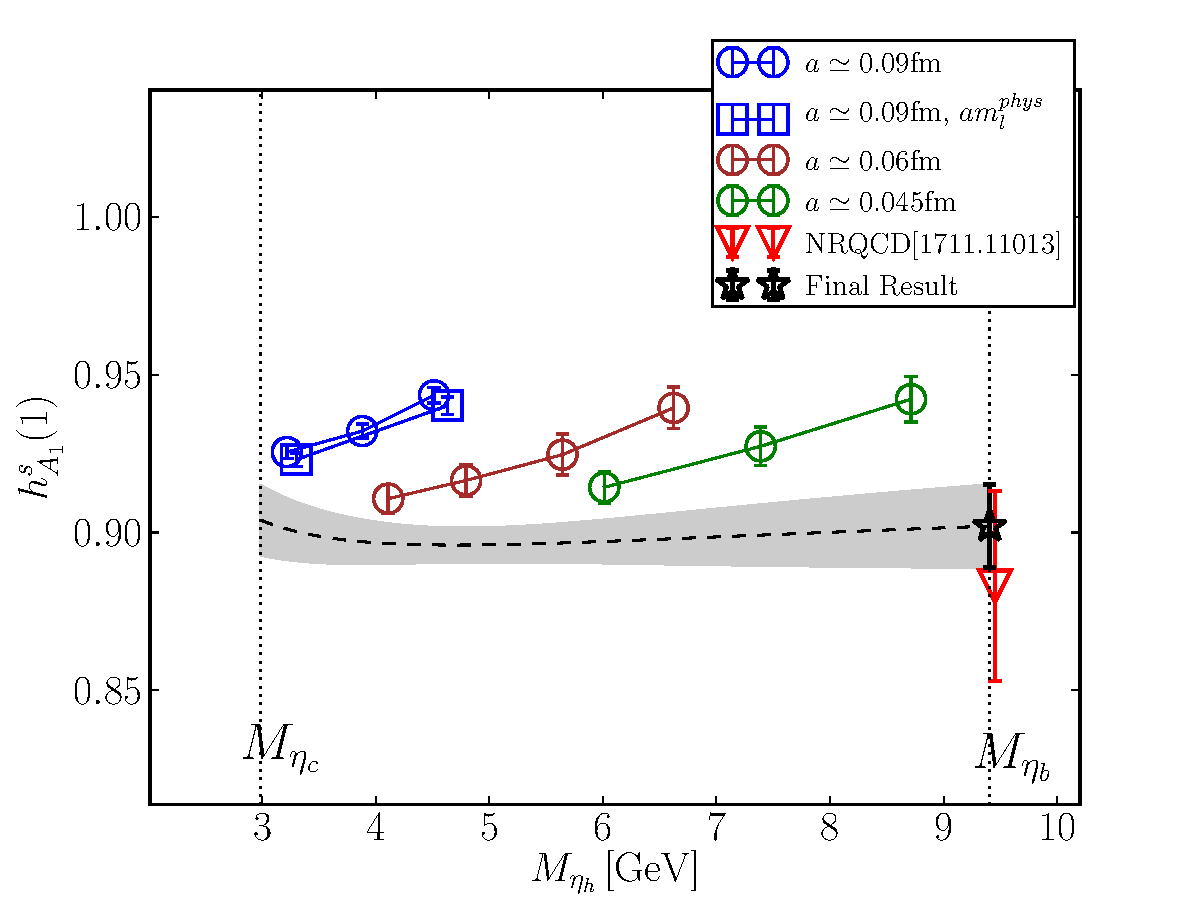
\includegraphics[width=0.90\textwidth]{images/BsDsstar/hA1_vsmh.pdf}
  \caption{ $h_{A_1}^s(1)$ against $M_{\eta_h}$ (a proxy for the heavy quark mass). The grey band shows the result of the extrapolation at $a=0$ and physical $l$,$s$ and $c$ masses. Sets listed in the legend follow the order of sets in table \ref{tab:BsDsensembles}. The red point represents a determination of the same quantity from a previous study using the NRQCD action for the $b$ \cite{Harrison:2017fmw}. \label{fig:hA1_vsmetah}}
  \end{center}
\end{figure}

\begin{table}
  \begin{center}
    \begin{tabular}{c c}
      \hline
      Source & \% Fractional Error \\ [0.5ex]
      \hline
      Statistics & 0.98  \\ [1ex]
      $a\to 0$ & 0.57  \\ [1ex]
      $m_h \to m_b$, $c$-mistuning & 0.36 \\ [1ex]
      $l$-mistuning & 0.08  \\ [1ex]
      $s$-mistuning & 0.03  \\ [1ex]
      \hline
      Total & 1.19 \\ [1ex]
      \hline
    \end{tabular}
  \end{center}
  \caption{Error budget for $h^s_{A_1}(1)$. \label{tab:errorbudget}}
\end{table}

Our result is statistics dominated. The systematic error is dominated by the continuum extrapolation. 

We include in fig. \ref{fig:hA1_vsmetah} a determination from the only other lattice determination of this quantity \cite{Harrison:2017fmw}. They report a value of $h_{A_1}^s(1) = 0.883(12)_{\text{stat}}(28)_{\text{sys}}$. Our two studies, containing independent systematic uncertainties, are in agreement.

This study used the same gluon ensembles, with HISQ $s$ and $c$ valence quarks, and an NRQCD $b$ quark. Using NRQCD meant they could perform their simulation directly at the physical $b$ mass. However, the matching of lattice NRQCD to continuum QCD causes their dominant error. Adding their errors from $\order{\alpha_s^2},\order{\alpha_s \Lqcd/m_b}$ and $\order{(\Lqcd/m_b)^2}$ corrections in quadrature, we find a 2.8\% error, while their total error is reported as 2.9\%.

\subsection{Extrapolation Stability}
\label{sec:stability}

We performed a number of tests of the continuum/heavy mass extrapolation. The results of each of these tests are given in fig. \ref{fig:fittests}.

\begin{figure}[htb!]
  \begin{center}
  \hspace{-18pt}
  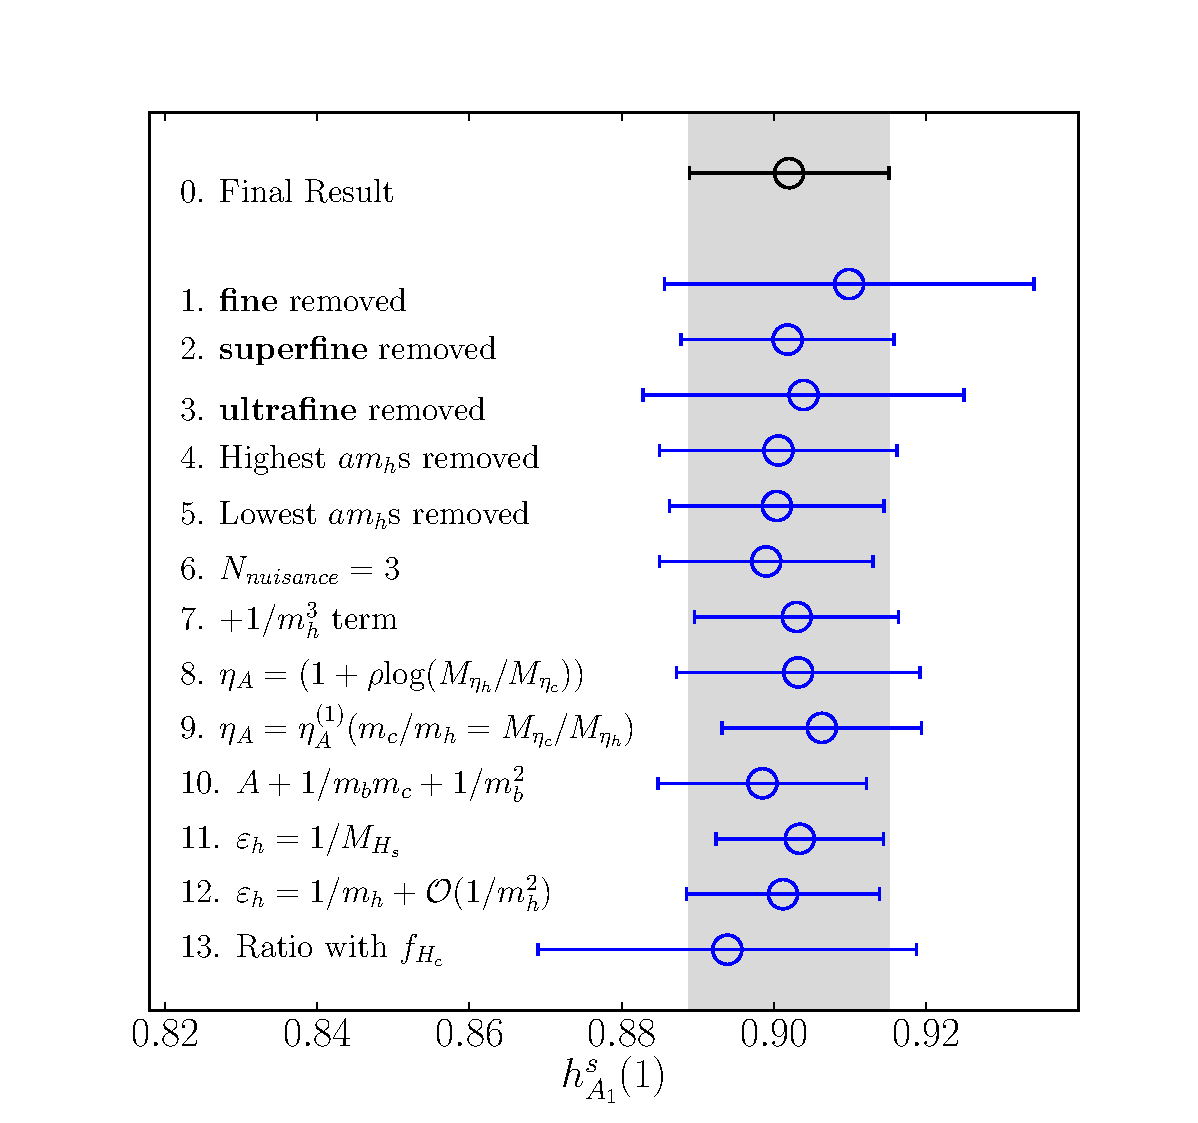
\includegraphics[width=0.8\textwidth]{images/BsDsstar/hA1vsmh_fittests.pdf}
  
  \caption{Results of $h_{A_1}^s(1)$ extrapolation tests. The top three blue points show $h_{A_1}^s(1)$ at continuum and physical $b$ mass, if data from the fine, superfine or ultrafine ensembles are not used in the fit. The fourth and fifth blue points show the result if data at the highest/lowest $am_{h0}^{\text{val}}$ value on each ensemble are removed. The point labelled 'No HQET input' is the result of a more naive heavy-mass extrapolation; the first line of \eqref{eq:fitform} is removed, and the sum in \eqref{eq:fitfun_hA1} is extended to include terms with $j+k=0$. An extra term to account for charm mass mistunings is added. The point labelled $N_{nuisance}=3$ is the result of extending the sum in \eqref{eq:fitfun_hA1} such that it truncates at 3 rather than 2 in each of the $i,j,k$ directions. The point labelled '$+1/m_b^3$' results from adding an extra term to \eqref{eq:fitform} of the form $p\varepsilon_h^3$ where $p$ is a fit parameter with the same prior as $l_{V,A,P}^s$. In this case, the Bayes factor falls by a factor of 7, suggesting that the data does not contain a cubic dependence on the heavy mass . The point labelled 'Ratio' is the result of an alternative extrapolation described in sec. \ref{sec:stability}.  \label{fig:fittests}}
    \end{center}
\end{figure}

One of the tests requires some explaination, the result of which is given in fig. \ref{fig:fittests}, labelled 'Ratio'. We performed a continuum/heavy mass extrapolation in the ratio $h_{A_1}^s(1)/(f_{H_c}\sqrt{M_{H_c}})$. $f_{H_c}$ is found from fitting the $H_c$ correlation functions to obtain $a_0^{H_c}$, and using eq. \eqref{eq:decayconstant_pseudoscalar}. Since we create the $H_c$ mesons with a local HISQ pseudoscalar current, which is absolutely normalized, no normalization of $f_{H_c}$ is required here. Details of the extrapolation are given in appendix \ref{sec:ratio_extrap}, and results are shown in fig. \ref{fig:fHc}. Discretization effects cancel to a large extent in this ratio, it however varies strongly with changing heavy mass. This makes the extrapolation very different to the extrapolation in $h_{A_1}^s(1)$, which has large discretization effects but has little variation in the heavy mass. Hence the two extrapolations have quite different systematics.

We also performed an extrapolation of $f_{H_c}$ to continuum and physical $b$, following precisely the methodology of \cite{McNeile:2012qf}, and sumarized in sec \ref{sec:ratio_extrap}. The result of the extrapolation of $h_{A_1}^s(1)/(f_{H_c}\sqrt{M_{H_c}})$ at continuum and physical $b$ mass was multiplied by our $f_{B_c}$ result, and the PDG value for $M_{B_c}$ \cite{PhysRevD.98.030001}, to obtain a second determination of $h_{A_1}^s(1)$. This is the result given in fig. \ref{fig:fittests} labelled 'Ratio'.

\begin{figure}[htb!]
  \begin{center}
  \hspace{-10pt}
  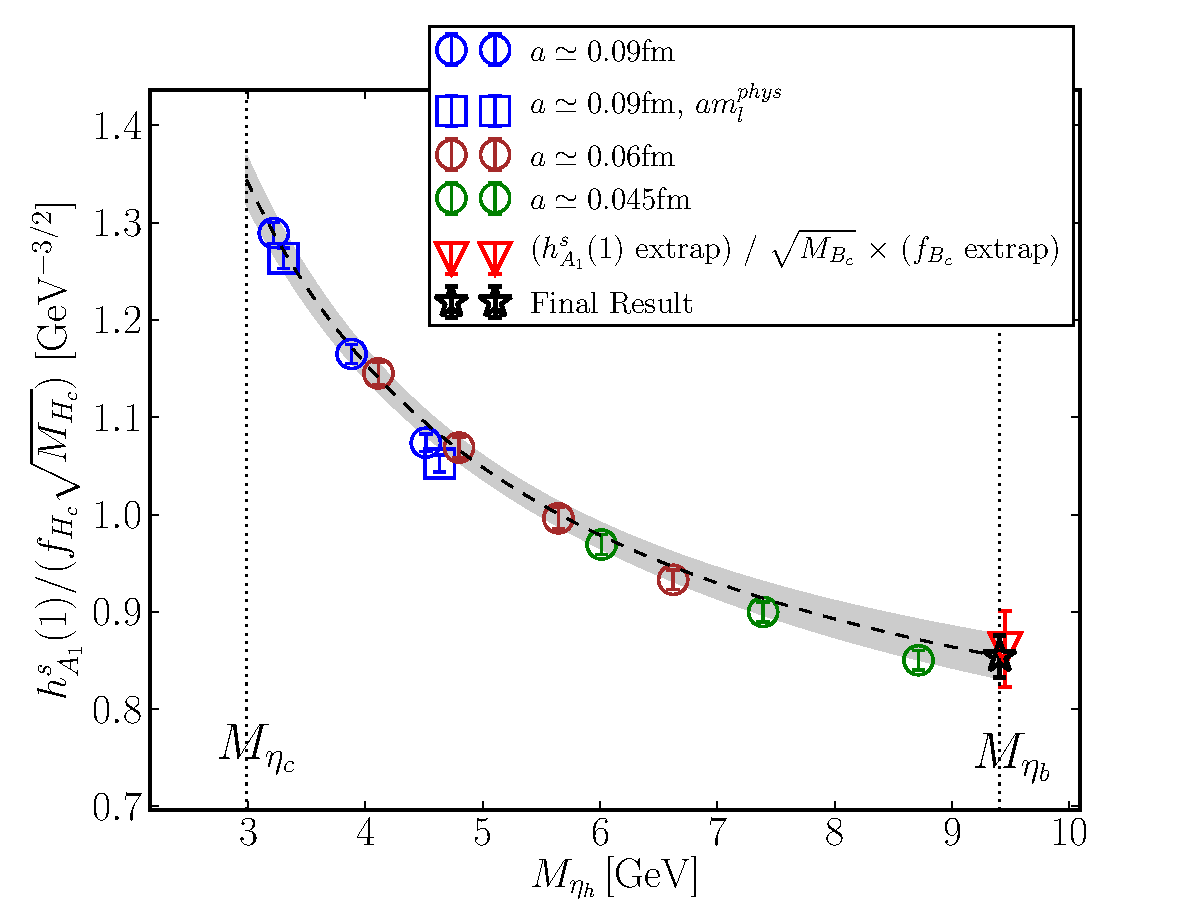
\includegraphics[width=0.85\textwidth]{images/BsDsstar/hA1overfHc.pdf}
  \caption{ $h_{A_1}^s(1)/(f_{H_c}\sqrt{M_{H_c}})$ against $M_{\eta_h}$ (a proxy for the heavy quark mass). The grey band shows the result of the extrapolation at $a=0$ and physical $l$,$s$ and $c$ masses. Sets listed in the legend follow the order of sets in table \ref{tab:BsDsensembles}. The black point shows our final result for $h_{A_1}^s(1)$ divided by $\sqrt{M_{B_c}}$ from the PDG \cite{PhysRevD.98.030001} and $f_{B_c}$ from our extrapolation of $f_{H_c}$ to continuum and physical $b$ mass. \label{fig:fHc}}
  \end{center}
\end{figure}

In fig. \ref{fig:comparison}, we show all current lattice results for $h_{A_1}(1)$ and $h_{A_1}^s(1)$. In fig. \ref{fig:fermilab_data}, we show lattice data from the previous FNAL/MILC and HPQCD, along with their final results, and the final result of this study, against 'pion mass'. Here pion mass refers to the mass of a pion containing quarks with the mass of the spectator quark. Here we can see that the FNAL/MILC lattice data is very flat in the spectator quark mass, so if they were to extrapolate their data to find $h^s_{A_1}(1)$, it would broadly be in agreement with out result.

\begin{figure}[htb!]
  \begin{center}
  \hspace{-20pt}
  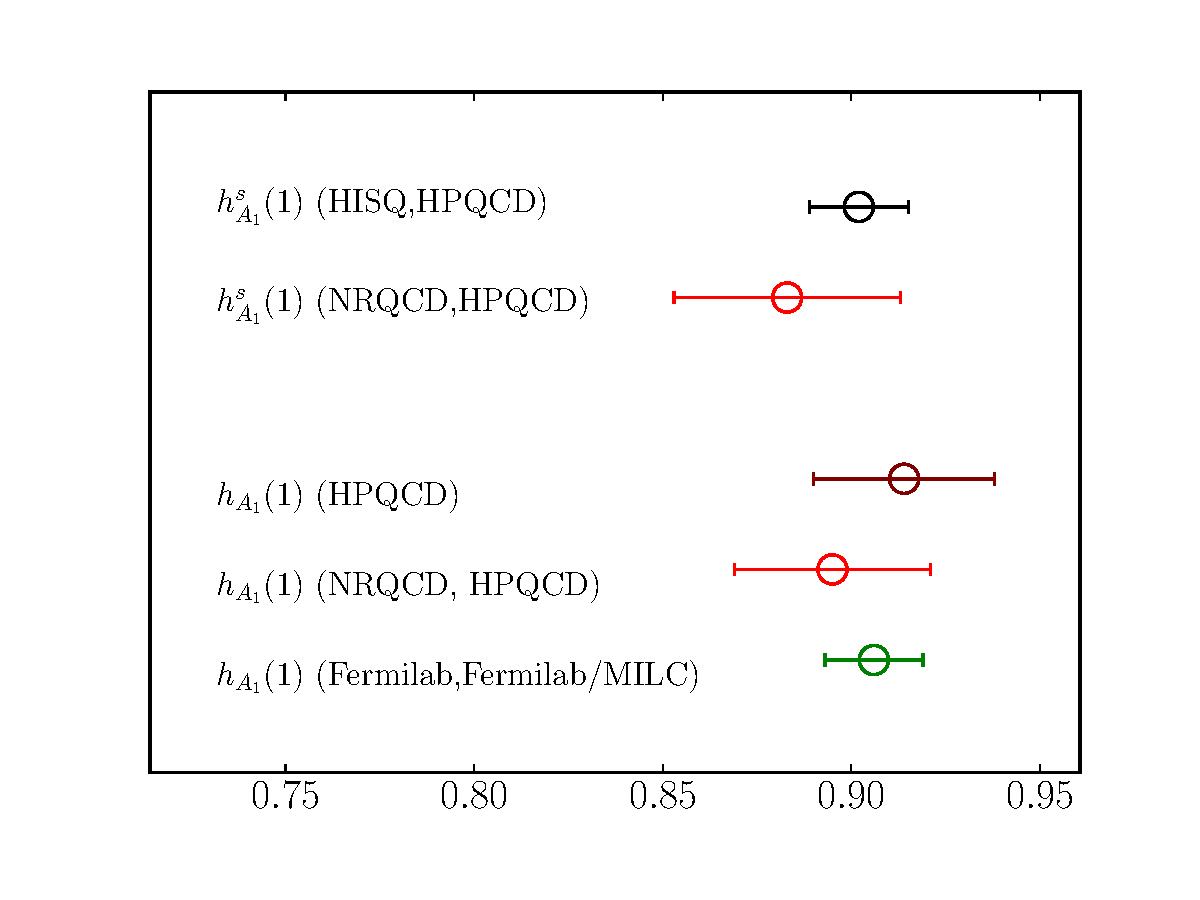
\includegraphics[width=0.7\textwidth]{images/BsDsstar/comparisons.pdf}
  \caption{ $h_{A_1}^{(s)}(1)$ from different calculations. Those marked (NRQCD,HPQCD) are from \cite{Harrison:2017fmw}. The quantity marked (this work \& NRQCD) is the result of multiplying our result for $h^s_{A_1}(1)$ with the ratio $h_{A_1}(1)/h^s_{A_1}(1)$ computed in \cite{Harrison:2017fmw}. The quantity marked (FNAL/MILC) is from \cite{Bailey:2014tva}. \label{fig:comparison}}.
  \end{center}
\end{figure}

\begin{figure}[htb!]
  \vspace{-20pt}
  \begin{center}
  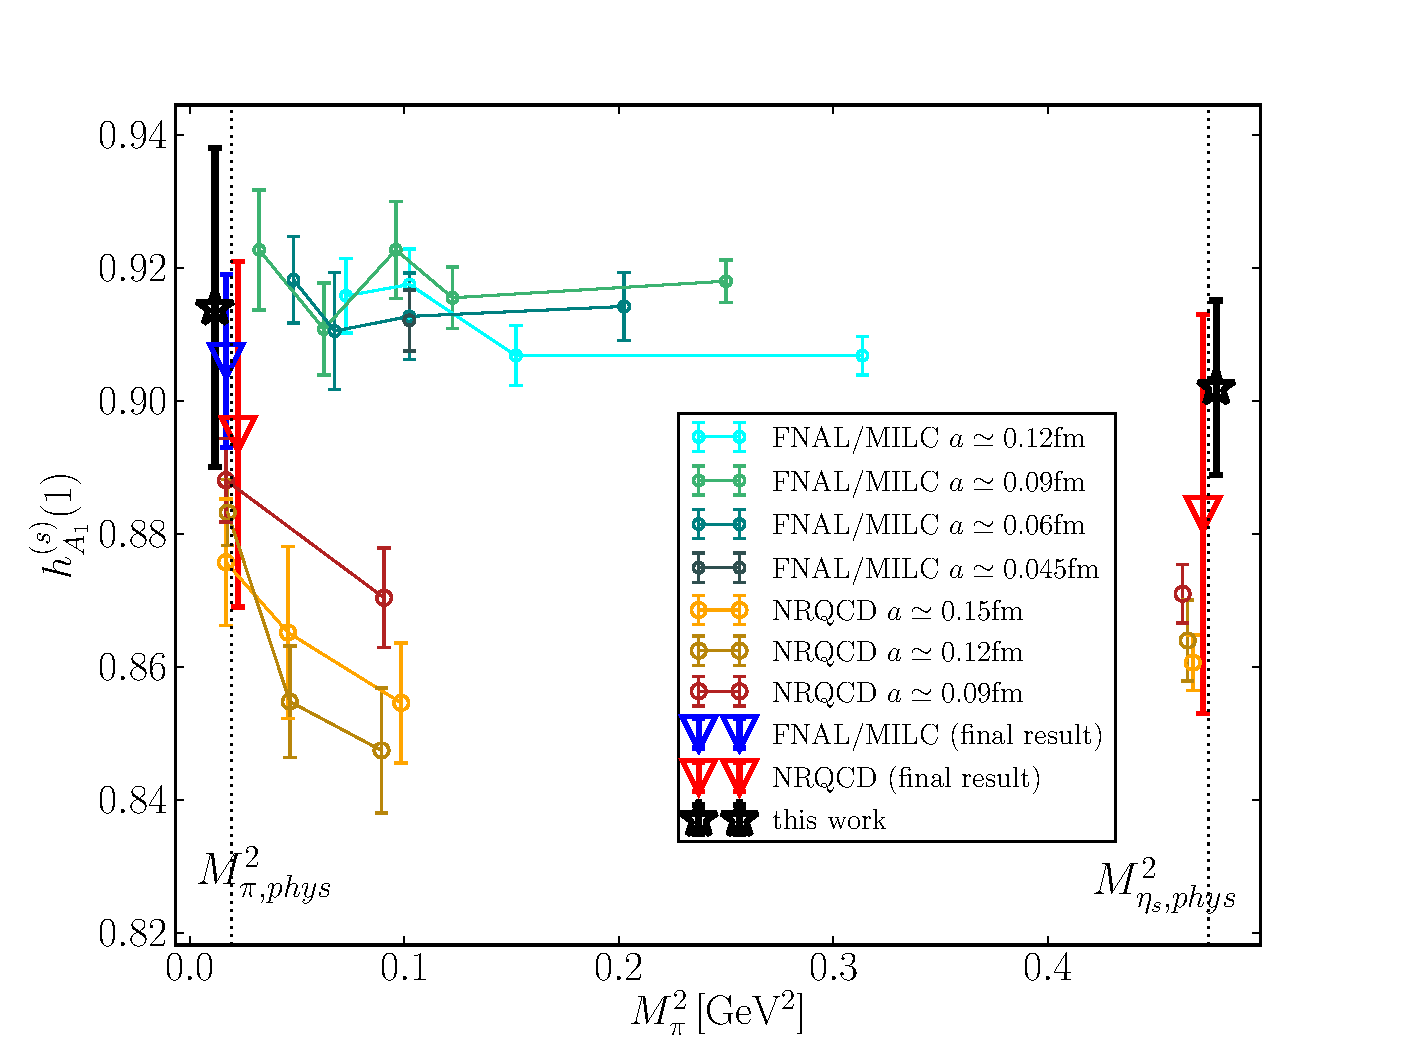
\includegraphics[width=1.2\textwidth]{images/BsDsstar/fermilab_nrqcd_data.pdf}
  \caption{Lattice data and continuum extrapolated data for three studies of $h_{A_1}(1)$ and $h_{A_1}^s$, against the pion mass. Points labeled FNAL/MILC are from \cite{Bailey:2014tva}, and those labeled NRQCD are from \cite{Harrison:2017fmw}. The x-axis must be taken with a pinch of salt, the points at $M_{\pi}=M_{\eta_s}$ have pions in the sea of smaller masses than $M_{\eta_s}$, but we place them here to signify that the spectator quark as the mass of a strange quark. \label{fig:fermilab_data}}
  \end{center}
  \vspace{-20pt}
\end{figure}

\subsection{Hints about $B\to D^*$}

As mentioned in the introduction, the $B_s\to D_s^*$ form factor seems to be very close to the equivalent $B\to D^*$ form factor. 

As an additional test of this claim, we obtained lattice data for $h_{A_1}(1)$ on the fine ensemble, for comparison with the $h_{A_1}^s(1)$ data within our formalism. This involved an identical process to that of obtaining $h_{A_1}^s(1)$, except with the strange valence quark replaced with a valence quark of a mass equal to $am_{l0}$, the sea light quark mass.

The $h_{A_1}(1)$ data is shown in comparison to the $h_{A_1}^s(1)$ data in fig. \ref{fig:BD_BsDs}. Errors are statistical. The error on $h_{A_1}(1)$ is much larger due to the presence of the valence light quark. There is no significant difference between $h_{A_1}(1)$ and $h_{A_1}^s(1)$ here.

\begin{figure}[htb!]
  \begin{center}
  \hspace{-10pt}
  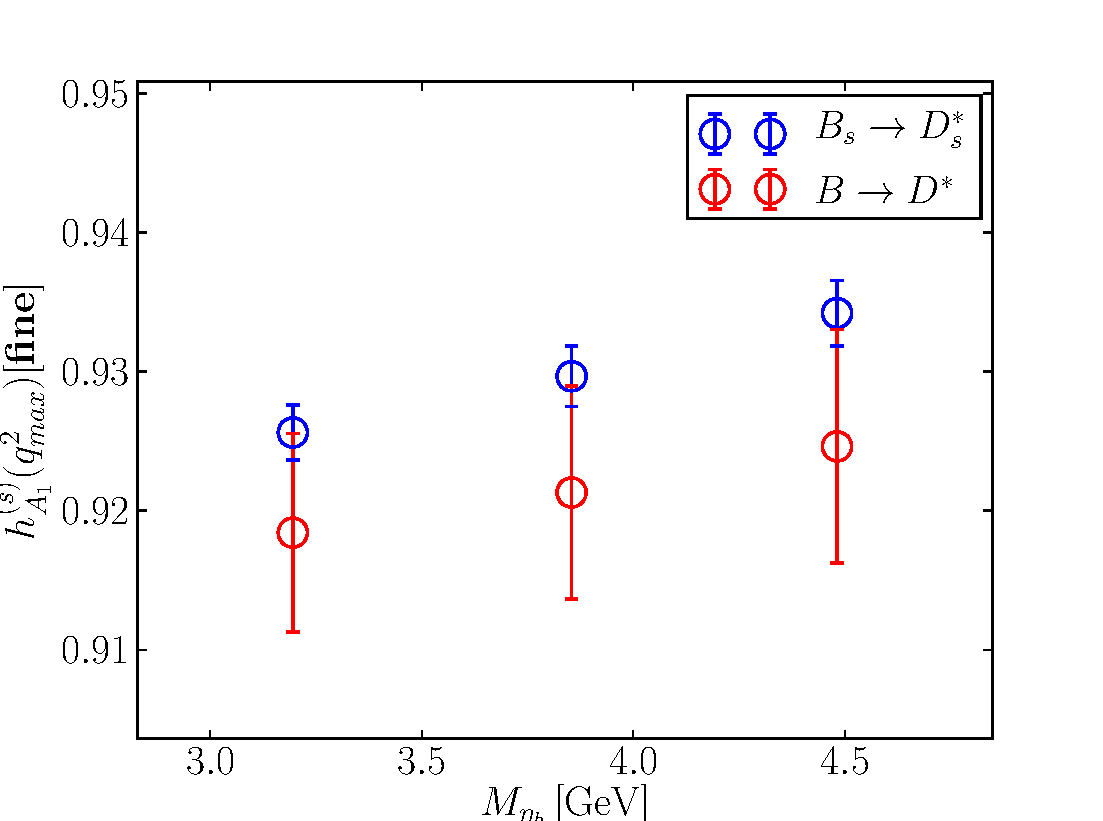
\includegraphics[width=0.7\textwidth]{images/BsDsstar/BD_BsDs.pdf}
  \caption{$h_{A_1}(1)$ and $h_{A_1}^s(1)$ data on the fine ensemble.\label{fig:BD_BsDs}}
  \end{center}
\end{figure}

In \cite{Harrison:2017fmw}, the ratio between these two quantities was computed - $h_{A_1}(1) / h^s_{A_1}(1) = 1.013(14)_{\text{stat}}(17)_{\text{sys}}$. Multiplying this by our result for $h^s_{A_1}(1)$, one finds a result consistent with the two previous $h_{A_1}(1)$ determinations.
\begin{align}
  \mathcal{F}^{B\to D^*}(1) = h_{A_1}(1) = 0.909(24).
  \label{eq:hA1_us_nrqcd}
\end{align}

\subsection{HQET Low Energy Constants}

\begin{table}
  \begin{center}
    \begin{tabular}{c c c c}
      \hline
      Source & $l^s_V$ & $l^s_A$ & $l^s_P$ \\ [0.5ex]
      \hline
      Statistics & 30.3 & 101.8 & 64.4  \\ [1ex]
      $a\to 0$ & 22.4 & 80.5 & 38.2 \\ [1ex]
      mistuning & 2.0 & 3.5 & 1.5  \\ [1ex]
      $\eta_A$ & 0.7 & 0.7 & 0.7 \\ [1ex]
      $\order{1/m_c^3}$ & 4.4 & - & -\\ [1ex]
      \hline
      Total & 40.0 & 136.9 & 78.9  \\ [1ex]
      \hline
    \end{tabular}
  \end{center}
  \caption{Error budget for HQET low energy constants. Each column gives the \% fractional error for the associated quantity. \label{tab:HQETbudget}}
\end{table}

Our fit of the lattice data to \eqref{eq:fitform} produced the fit parameters $l^s_{V,A,P}$, which as discussed in sections \ref{sec:BsDsstar_heavymass} and \ref{sec:massambiguities}, are numerically equal to the low energy HQET constants of the same name. We find
\begin{align}
  \nonumber  l^s_V &= 0.59(24)\text{GeV}^2, \\  l^s_A &= -0.08(11)\text{GeV}^2, \label{eq:hqet_constants}
  \\ \nonumber l^s_P &= -0.25(20)\text{GeV}^2.
\end{align}
% These are the first lattice determinations of these quantities. %Not sure if this is true!!
Since the lattice data contains all orders of HQET, $l_V$ has been given a systematic uncertainty due to contamination from higher orders in $1/m_c$. Accordingly a systematic error of size $(\varepsilon_c \Lambda_{\text{QCD}})^3 \simeq 0.03$ is included in the $l_V$ result. We also include an error accounting for the error in $\eta_A$ that we neglect in the fit.

An estimate from the ISGW model for $B\to D^*$ decays gives \cite{PhysRevD.39.799}
\begin{align}
  l_P \simeq l_V \simeq 0.39\text{GeV}^2.
\end{align}
One does not expect these to differ significantly from $l_{V,A,P}^s$. These are of the same order of magnitude as our results. It is notable however that we find a different sign for $l_P$ to the ISGW result.

\subsection{Extrapolation of $h_{A_1}^s(1)/(f_{H_c}\sqrt{M_{H_c}})$ and $f_{H_c}$}
\label{sec:ratio_extrap}

As a consistency test of our result we also perform extrapolations in $h_{A_1}^s(1)/(f_{H_c}\sqrt{M_{H_c}})$ and $f_{H_c}$, then combine them to find a second determination of $h_{A_1}^s(1)$.

Both extrapolations use a fit function of the form
\begin{align}
  \label{eq:fitfun_ratio}
  \nonumber
  \text{fit} = &\left({\alpha_s(M_{\eta_h})\over\alpha_s(M_{\eta_c})}\right)^p M_{\eta_h}^{n/2} \times \\ &\sum_{i,j,k=0}^{2,2,2} d_{ijk} \left({\Lambda_{\text{QCD}}\over M_{\eta_h} }\right)^{i} \left({ am^{\text{val}}_{h0} \over \pi }\right)^{2j} \left({ am^{\text{val}}_{c0} \over \pi }\right)^{2k} \\
  &+ \mathcal{N}_{\text{mistuning}}.
  \nonumber
\end{align}
$\alpha_s(M)$ is the QCD coupling constant evaluated at scale $M$. $p$ is a fit parameter with prior distribution $\pm2/9\pm 1/9$, $+$ for $h_{A_1}^s(1)/(f_{H_c}\sqrt{M_{H_c}})$ and $-$ for $f_{H_c}$. $n=0$ for $h_{A_1}^s(1)/(f_{H_c}\sqrt{M_{H_c}})$ and $n=-1$ for $f_{H_c}$. The $M_{\eta_h}^{n/2}$ accounts for the leading order dependance of $f_{H_c}$ in HQET, and the $\alpha_s$ ratio comes from matching between QCD and HQET of $f_{H_c}$. $\mathcal{N}_{\text{mistuning}}$ is defined in \ref{eq:mistuning}.

The extrapolation in $f_{H_c}$ is shown in fig. \ref{fig:fHc_vsmh}. We here include the result from a previous heavy-HISQ determination of $f_{B_c}$ on 2+1 gauge ensembles \cite{McNeile:2012qf}. Our result is slightly higher than theirs, since their study used only unphysically heavy light quarks ($m_l/m_s\simeq=0.2$), and did not control for associated effects. Our final result for this quantity is
\begin{align}
  f_{B_c} = 0.4350(55).
\end{align}

\begin{figure}[htb!]
  \begin{center}
  \hspace{-20pt}
  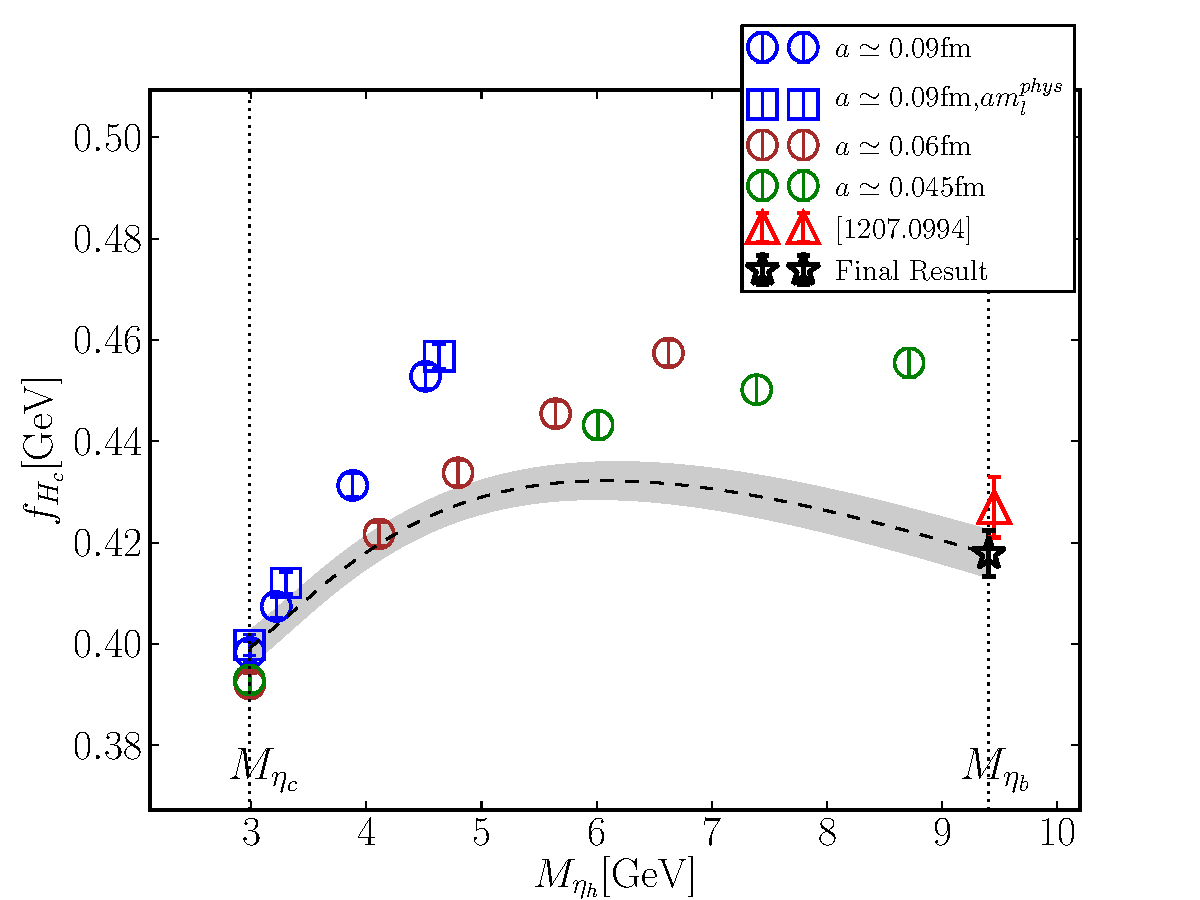
\includegraphics[width=0.90\textwidth]{images/BsDsstar/fHcvsmh.pdf}
  \caption{ $h_{A_1}^s(1)$ against $M_{\eta_h}$ (a proxy for the heavy quark mass). The grey band shows the result of the extrapolation at $a=0$ and physical $l$,$s$ and $c$ masses. Sets listed in the legend follow the order of sets in table \ref{tab:BsDsensembles}. The red point shows the result from a previous heavy-HISQ determination of $f_{B_c}$ on 2+1 gauge ensembles \cite{McNeile:2012qf}\label{fig:fHc_vsmh}}.
  \end{center}
\end{figure}

\section{Conclusions}
\label{sec:conclusions}

We have produced a fully non-perturbative determination of $h_{A_1}^s(1)$, sometimes called $\mathcal{F}^{B_s\to D_s}(1)$, using unquenched lattice data from a fully relativistic and highly improved lattice action, along with the low energy constants $l_{V,A,P}^s$, given in \eqref{eq:finalresult} and \eqref{eq:hqet_constants} respectively. We used gauge ensembles with 3 lattice spacings, including an ensemble with approximately physical light sea quark masses, and obtained data corresponding to 12 different heavy quark masses.

This study supplies an independent check of the NRQCD formalism used in previous HPQCD studies. It is also much more precise, in the case of $h_{A_1}^s$, the total fractional error has been halved in comparison to the NRQCD determination. The comparative precision resulting from the heavy-HISQ method suggests that it is well suited to computing other form factors associated with $b$-decays. A sister paper, studying the $B_s\to D_s$ form factors throughout the physical $q^2$ range, is in progress.

Various improvements to this study could be implemented in future calculations. For example - since the uncertainty is dominated by statistics, more lattice data should be included. One useful innovation that was not used here is the Covariant Approximation Averaging approach to solving quark propagators \cite{PhysRevD.91.114511}, this could significantly boost statistics while keeping computational cost manageable.
%%
